% https://sites.google.com/vols.utk.edu/rewords23/home
\PassOptionsToPackage{hyphens}{url}
\documentclass[conference]{IEEEtran}
\IEEEoverridecommandlockouts

% The preceding line is only needed to identify funding in the first footnote. If that is unneeded, please comment it out.


\usepackage{cite}
\usepackage{amsmath,amssymb,amsfonts}
\usepackage{algorithmic}
\usepackage{graphicx}
\usepackage{textcomp}
\usepackage[dvipsnames]{xcolor}
\usepackage{comment}
\usepackage[hidelinks]{hyperref}
\usepackage{fancyvrb}
\usepackage{fvextra}
\usepackage{xcolor}

\PassOptionsToPackage{hyphens}{url}
\pdfoutput=1

\usepackage[pdf]{graphviz}

\usepackage{fancyvrb}
\newcommand{\TODO}[1]{\begin{quote}\color{red}{\em TODO:}{\bf #1}\end{quote}}
\newcommand{\DONE}[1]{{\color{PineGreen}{\bf\em DONE:} #1}}
\newcommand{\SPACE}[1]{{\color{blue}{\bf\em SPACE:} #1}}


\renewcommand\IEEEkeywordsname{Keywords}
\newcommand{\orcidicon}[1]{\href{https://orcid.org/#1}{
\includegraphics[width=9pt]{orcid_icon}}}

% \usepackage{color}
\usepackage{listings}
% \usepackage{xcolor}
% \usemintedstyle{trac}
% \definecolor{mblue}{rgb}{0.27,0.33,0.53}

\lstset{
  basicstyle=\fontsize{6}{6}\ttfamily,
  breaklines=true,
  keywordstyle=\color{BrickRed},
  moredelim=[s][\color{BrickRed}]{\{}{\}},
  % moredelim=[s][\bfseries]{workflow:}{\n},
  % moredelim=[s][\bfseries]{nodes:}{\n},
  % literate={\{}{{\textbf{\{}}}1
  % literate={workflow:}{{{\bfseries workflow:}}}9,
  % literate={nodes:}{{{\bfseries nodes:}}}6,
  escapeinside={(*}{*)}
}

% these do not use shell escape!
% therefore they are arxiv safe

\lstdefinestyle{python}{
  language=Python,
  basicstyle=\scriptsize\ttfamily,
  keywordstyle=\color{blue},
  commentstyle=\color{green!50!black},
  stringstyle=\color{Bittersweet},
  showstringspaces=false,
  breaklines=true
}

\lstdefinestyle{sh}{
  language=sh,
  basicstyle=\scriptsize\ttfamily,
  keywordstyle=\color{blue},
  commentstyle=\color{green!50!black},
  stringstyle=\color{Bittersweet},
  showstringspaces=false,
  breaklines=true,
  keywords={singularity,echo}
}

% \lstdefinestyle{yaml}{
%   keywordstyle=\bfseries\color{blue},
%   moredelim=[s][\bfseries\color{blue}]{workflow:}{\n},
%   moredelim=[s][\bfseries\color{blue}]{nodes:}{\n}
% }

\definecolor{friendlybg}{HTML}{f0f0f0}
\definecolor{lightgray}{rgb}{.9,.9,.9}
\definecolor{darkgray}{rgb}{.4,.4,.4}
\definecolor{purple}{rgb}{0.65, 0.12, 0.82}

    
\begin{document}
%\pagenumbering{Roman}
%
\newcommand{\OK}{$\checkmark$}
\newcommand{\ok}{$\checkmark$}

{\bf done. Gregor registered} Each paper is required to have one author register for eScience using the author rate. https://www.escience-conference.org/2023/registration


The camera ready version is due in a few days (14 August 2023). 

----------------------- \OK \DONE{REVIEW 1} ---------------------

\begin{itemize}
\item  \ok \DONE{}The authors mention that it is easily adapted to other applications, are those applications exclusively from the MLsCommons benchmarks?

see aprox. line 955. added citations \cite{las-22-arxiv-workflow-cc,las-22-mlcommons-science}


\item \OK \DONE{} {\bf no space, should be added to larger paper} Related work section is really short. WfCommons is a framework for scientific workflows and also has a human-readable description of the workflows called WfFormat. There are many workflow management systems that could have been cited here for comparison (Pegasus, Kepler, etc..) Also our framework we developed existed before WfCommons as far as we know.

\item \OK \DONE{6-11 are very small and hard to read}

\item \OK \DONE{was already fixed, but not in submitted version} Section V has a typo: "As it uses templated virtual machine specification sit s easy to switch from one"

\item \OK \DONE{} In Section IV, item C, the sentence: "In Figure ?? we showcase the execution of an experiment that combines the Cloudmesh.." the number of the figure did not come out. 

\item \OK \DONE{} Section IV. In the same section, when talking about the experiment configuration, the authors say that the epochs are 1, 30 and 40, but in the code snippet, the epochs are set to 1, 30 and 60.

\item \OK \DONE{added to conclusion.} The conclusion contains no future work/improvements/next steps, which brings some questions:

\begin{itemize}
\item \OK Are you going to run in bigger setups with more  HPC machines/ desktops/ cloud systems to evaluate the efficiency of your management system?

\item \OK What if the application is data-driven? What about latency caused by IO operations?

\item \OK What about  Communication/scheduling overhead for larger and more heterogenous set-ups? 

\item \OK Those are all good future directions that could be explored with your management system.

\end{itemize}

\end{itemize}


----------------------- \OK \DONE{REVIEW 2} ---------------------


I see two main contributions from this work: 

1) \OK the experiment execution that allows the users to iterate over different parameters for the scientific application to find the optimal set of parameters with the templated configurations and 

2) \OK the claim of simplicity and execution portability of the framework.

\DONE{do to space limitations this can not be elaborated on much. } 

 I think that given the space the authors limited adding information that could have provided a much clearer picture of the work and project. 

 
 
 3) \OK The authors decide that it is out of the scope to mention many different workflow systems but it is key to provide a comparison of the novel aspects of this framework compared to other efforts in HPC and in Cloud of workflow management platforms  (e.g., Pegasus, Galaxy, Airflow, Argo workflows, Kubeflow) that also offer interactive ways of designing and executing scientific workflows on hybrid resources. 

\OK \DONE{A reference to a much larger paper is provided, that however is not yet published on arxiv. This was the version originally submitted, but was 10 pages long and needed to be cut to 5 pages.}
 

\begin{itemize}

 \item \OK Another concern I have is in terms of storing the executed program and its output, what are the impacts in terms of resources for storing all this information? 

 \DONE{Section IV.C. dded prediction sentence}
 
 \item \OK Are there ways to filter or curate the data that is being saved? 

 \SPACE{Scripts have been developed as templates to mine the data produced. HOwever they are not as of yet part of the framework, but can be copied from the application. There is no space to describe this in detail.}
 
 \item \OK Also, there are some very vague claims about how the EE has significantly reduced the time for benchmarking but there is no clear experimental demonstration of this claim. 

\SPACE{Due to space we can not give more details than this sentence. It has been used by multiple students, where 5 students did not use it while two students did use it. One of two switched to the framework as the program previously developed did not work as expected and introduced complexities into running the code that immediately could be resolved by the framework. Whenever we look at an application (by now 6) we find that using the framework simplifies things.}
 
 \item \OK The use case section shows how the framework compares the runtime on different GPUs and the collection of hyperparameters but there is not a users perspective in terms of the integration of the workflow to the framework, additionally what are the efforts to adjust the hyperparameters and interface to your specific application. 

\DONE{we added this is done for runtime predictions which is more elaborated on in the larger paper.}
\SPACE{Space issues prevent us to write abut here in more detail.}
 
 
 \item \OK Finally, what are the future steps of the project, what type of reusability efforts from user to user are available in the framework. 

\DONE{We added some future steps while focusing on applications}

\item \OK link to the GitHub repository. 

\DONE{create and update cloudmesh-ee, include as reference.}

\item \OK \DONE{} I think the authors need to motivate more the unique contributions of this workflow and why do we need to create a new one, already being invaded by many systems. 

\SPACE{This is part of the paper, and in more detail elaborated in the 10 page original paper.}

\TODO{Maybe: full stateless and state control is implemented within the queuing system or execution engine. state is communicated through simple print statements in log files that are monitored with pull requests. The system is completely restartable which is important for jobs that run many days. This is in the conclusion , but may need to be added elsewhere.}

\item \OK \DONE{} In page 4, column 2 paragraph 1, there is an unlinked figure 


\item \OK \DONE{paper is no longer 5 pages, but 6} Some figures are unreadable when the paper is printed

\item \OK \DONE{not implementable. IEEE format specifically says figures must be used. see X. B. in guidelines.} Some figures (2 and 3 and the configuration file for cloudmask) should be code listings 


\end{itemize}
\end{itemize}

----------------------- REVIEW 3 ---------------------
The paper is a good fit for the rewords workshop and describes and offers a solution many computational scientists and machine learning practitioners face. 

\begin{itemize}

\item \OK \DONE{} The system is advertised to also extend to the cloud but it is not demonstrated in the evaluation.
    
\item \OK \DONE \SPACE{not focus of this paper, but potentially another paper with project that does benchmarks on AWS but not for MLComons} 


\item \OK The structure and editing and the paper could be improved. While many important challenges are raised and sometimes detail is provided, 
the consequences for the design or why a detail was shared is sometimes unclear putting a lot of burden on the reader to puzzle together.}

\SPACE{Others commented paper is easy to understand. However do to space restrictions we needed to cut a lot of text}

\item \OK The introduction, talks at great length about MLCommons, which is a fantastic initiative, but besides the affiliation of the activities, it is not clear how insights and access to the MLCommons helped refine the designs. 

\OK \DONE{The framework is applied to aspiering researchers and not just MLCommons experts. THis is where the design requirements focus and is explained in the paper. }

\TODO{motivate more that we do not just do a regular workflow but a workflow doing FAIR principle based reproducible workflows. Mention however the framework can be used for any task requiring orchestration on HPC and cloud systems.}

\item \OK Two possible connection points seem to be Page 2, Section II, B, 1) mentions that best practices and needed features for workflow specification maybe learned from the past, and I could imagine MLCommons may have helped here, but in the current manuscript it is just a claim, that would benefit from additional context. 

\SPACE{no space to present more then the claim?. We have worked on workflows since 1989 and many best practices have been ntecrated from our decades long experience. However many other frameworks exist. We focus her enot on a general Workflow Framework but on how we can execute experiments in reproducible fashion.}

\item \OK Similarly, you note experiences and challenges with students and emphasize also focusing on the needs for educational context when defining these workflows. Some more details to understand in how far these experiences were quantified would be helpful.

\SPACE{mention experience was gathered while observing students from at least 5 universities and their struggle to get benchmarks established on the HPC systems dealing with software carpeting, HPC access, and introduction to Deep Learning. Students were participating in an NSF sponsored REU. Cite cybertraining.}

\item \OK Similarly, I think the requirements section could be sharpened. For example, Section II, A 1) and 2) formulate clear requirements in the description while 3) and 4) seem to enumerate modes of operation rather than refining the requirement.

\DONE{The operation is part of the design requirements. I think the reviewer had design of workflow in mind while we have architectural requirements in mind. Maybe we switch to Workflow Design requirements and Operational requirements.

Resolution: We added the term architecture design requirement to make it clear.
} 

\item \OK For Section II, B, 3, you identify monitoring as an important requirement, but later also begin discussing timers, potentially for performance. I would extend the workflow monitoring requirement beyond the aspects of orchestration and tracking progress to also include performance.

\DONE{Added the word state and performance monitoring as in our understanding of monitoring it includes both classes}

\item \OK On page 4, you write “We have defined a special status progress update specification that is universally applicable.” could you elaborate? Given the complexity and the integration across the systems you list, what mechanisms are you using to be universal?

\SPACE{added through files incl stdout and stderr}

\item \OK Also on page 4 you use lines of code as a metric for the simplicity requirement. But it is not clear if this refers to the LOC for your framework or the workflow you later run. Given the context, I would assume the framework, but the burden for users is not in the complexity of the framework implementation, but rather the changes and boilerplate they need for their workflow, and the number of concepts and features they have to familiarize themselves with to use your system effectively.

\DONE{It applies to both. it is important that the framework be small so students can participate and contribute}

\item \OK \DONE{} There is a minor typo in Section II, A. 3) where I believe it should say “Services”

\end{itemize}

%\pagenumbering{arabic}
%\setcounter{page}{0}


\title{Templated Hybrid Reusable Computational Analytics Workflow Management with Cloudmesh, Applied to the Deep Learning MLCommons Cloudmask Application\thanks{Funded by NSF, DOE, NIST, and University of Virginia. In part funded by the NSF CyberTraining: CIC:
CyberTraining for Students and Technologies from Generation Z with the
award numbers 1829704 and 2200409 and NIST 60NANB21D151T.}
}
  
\author{\IEEEauthorblockN{1\textsuperscript{st} Gregor von Laszewski}
\IEEEauthorblockA{\textit{Biocomplexity Institute}\\
\textit{University of Virginia}\\
Charlottesville, VA 22911, USA \\
laszewski@gmail.com \\
0000-0001-9558-179X}
\and
\IEEEauthorblockN{2\textsuperscript{nd} J.P. Fleischer}
\IEEEauthorblockA{\textit{Biocomplexity Institute}\\
\textit{University of Virginia}\\
Charlottesville, VA 22911, USA \\
jacquespfleischer@gmail.com \\
0000-0002-1102-1910}
\and
\IEEEauthorblockN{3\textsuperscript{rd} Geoffrey C. Fox}
\IEEEauthorblockA{\textit{Biocomplexity Institute}\\
\textit{University of Virginia}\\
Charlottesville, VA, USA \\
gcfexchange@gmail.com \\
0000-0003-1017-1391}
\and
\IEEEauthorblockN{4\textsuperscript{th} Juri Papay\\
5\textsuperscript{th} Sam Jackson \\
6\textsuperscript{th} Jeyan Thiyagalingam }
\IEEEauthorblockA{\textit{Rutherford Appleton Laboratory}\\
Harwell Campus\\
Didcot, OX11 0QX, UK\vspace{-2cm}}
%{\vspace{-0.2cm}\scriptsize
%{juri.papay,samuel.jackson,t.jeyan\}\\
%{\scriptsize @stfc.ac.uk}}
}



\maketitle
% -------------------------------
% remove this for no page numbers
\thispagestyle{plain}
\pagestyle{plain}
% -------------------------------

\begin{comment}
The CloudMask benchmark is a large-scale application both in terms of data size and computational load, therefore it is often used as a test case for measuring the scalability and performance of distributed learning. The data comes from the Sea and Land Surface Temperature Radiometer (SLSTR) instrument deployed on the Sentinel-3 satellite. For a clear sky this instrument can measure the Sea Surface Temperature (SST) accurately, however, when the sky is overcast the data becomes unreliable. Therefore it is essential to determine the presence of clouds for each individual pixel of the satellite image. This operation is referred to as {\em cloud masking}, i.e. classifying each individual pixel into two categories {\em clear sky} or {\em cloud}. This can be a challenging task since there are other phenomena that might look like clouds, for example, smoke from fires, dust storms, and sea ice which the network should be able to detect.

The benchmark uses a U-Net which is a deep neural network model with over two million trainable parameters \cite{unet}. The input includes two datasets with 180GB and 2.3TB, respectively. Each dataset is made up of two parts: reflectance and brightness temperature. The reflectance is captured across six channels with the resolution of 2400 x 3000 pixels, and the brightness temperature is captured across three channels with the resolution of 1200 x 1500 pixels. The output is a single-channel image with the same size as the input image with probabilities indicating whether the pixel is a cloud (Figure \ref{fig:satelite}).


\begin{figure}[htb]
\vspace{-0.5cm}
\begin{minipage}[t]{0.49\columnwidth}
\centering  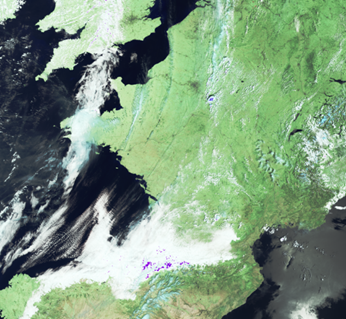
\includegraphics[width=1.0\columnwidth]{images/image002.png}
%\caption{Table view.}
%\label{fig:table-view}
\end{minipage}
\hfill
\begin{minipage}[t]{0.49\columnwidth}
  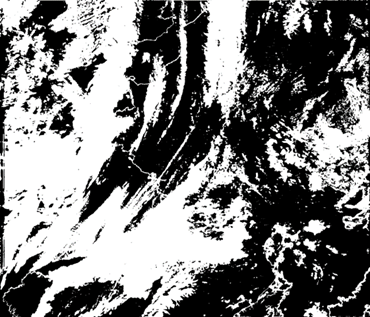
\includegraphics[width=1.0\columnwidth]{images/image004.png}
\end{minipage}
 \caption{
 (left) Raw image from the Sentinel-3 satellite, (right) Predicted probability that a particular pixel is a cloud.}
\label{fig:satelite}
\end{figure}
 
\end{comment}



\begin{abstract}
 
 In this paper, we summarize our effort to create and utilize an {\em
 integrated} framework to coordinate computational AI analytics tasks with
 the help of a task and experiment management workflow system. Our design is based on a minimalistic
 approach while at the same time allowing access to hybrid
 computational resources offered through the owner's computer, HPC
 computing centers, cloud resources, and distributed systems in
 general. Access to this framework includes a GUI for
 monitoring and managing the workflow, a REST service, a command line
 interface, as well as a Python interface. 
 It uses a template-based batch management system that, through configuration files, easily allows 
 for the generation of reproducible experiments while creating permutations over
 selected experiment parameters as typical in deep learning applications. The resulting framework was
 developed for analytics workflows targeting MLCommons benchmarks of AI
 applications on hybrid computing resources, as well as an educational tool
 for teaching scientists and students sophisticated concepts to
 execute computations on resources ranging from a single computer to
 many thousands of computers as part of on-premise and cloud
 infrastructure. We demonstrate the usefulness of the tool while
 creating FAIR principle-based application accuracy benchmark generation for the MLCommons
 Science Working Group Cloudmask application. The code is available as
 an open-source project in GitHub and is based on an easy-to-enhance
 framework called Cloudmesh. It can be applied to other applications easily.
\end{abstract}

\begin{IEEEkeywords}
experiment workflow, task workflow, hyperparameter workflow, high-performance computing, batch queue management, workflow web service. 
\end{IEEEkeywords}



% \section{Introduction}




%\renewcommand{\shortauthors}{von Laszewski, et al.}



% 
\begin{CCSXML}
<ccs2012>
<concept>
<concept_id>10010520.10010521.10010537</concept_id>
<concept_desc>Computer systems organization~Distributed architectures</concept_desc>
<concept_significance>500</concept_significance>
</concept>
<concept>
<concept_id>10010520.10010521.10010537.10003100</concept_id>
<concept_desc>Computer systems organization~Cloud computing</concept_desc>
<concept_significance>500</concept_significance>
</concept>
<concept>
<concept_id>10011007.10010940.10010971.10011120</concept_id>
<concept_desc>Software and its engineering~Distributed systems organizing principles</concept_desc>
<concept_significance>500</concept_significance>
</concept>
</ccs2012>
\end{CCSXML}

\ccsdesc[500]{Computer systems organization~Distributed architectures}
\ccsdesc[500]{Computer systems organization~Cloud computing}
\ccsdesc[500]{Software and its engineering~Distributed systems organizing principles}

\keywords{high performance computing, batch queue, service}




%\begin{CCSXML}
%<ccs2012>
%<concept>
%<concept_id>10010520.10010521.10010537</concept_id>
%<concept_desc>Computer systems organization~Distributed architectures</concept_desc>
%<concept_significance>500</concept_significance>
%</concept>
%<concept>
%<concept_id>10010520.10010521.10010537.10003100</concept_id>
%<concept_desc>Computer systems organization~Cloud computing</concept_desc>
%<concept_significance>500</concept_significance>
%</concept>
%<concept>
%<concept_id>10011007.10010940.10010971.10011120</concept_id>
%<concept_desc>Software and its engineering~Distributed systems organizing principles</concept_desc>
%<concept_significance>500</concept_significance>
%</concept>
%</ccs2012>
%\end{CCSXML}

%\ccsdesc[500]{Computer systems organization~Distributed architectures}
%\ccsdesc[500]{Computer systems organization~Cloud computing}
%\ccsdesc[500]{Software and its engineering~Distributed systems organizing principles}

% \keywords{high performance computing, batch queue, service}



%\received{20 February 2007}
%\received[revised]{12 March 2009}
%\received[accepted]{5 June 2009}

% set page numbers
% \settopmatter{printfolios=true}

\maketitle

% \FILE{cc.tex}

\section{Introduction}

In this section we provide an introduction to our work while
moving forward to motivate a 
Hybrid Reusable Computational Analytics Workflow
Management Framework.

\subsection{Reusable Computational Analytics}

{\em Reusable computational analytics} (RCA) focuses on the creation of reusable programs, patterns, and services to conduct analytics tasks that are part of the scientific discovery process. RCA service need varies widely and may include multi-scale hardware resources as well as multi-scale scientific applications. To utilize such services and their resources in a reusable way, we need to have a mechanism to express them in an easy fashion that goes beyond just the definition in one programming language or framework, but allows the integration into many different programming languages and frameworks so that services that may be designed in one framework or language may be reusable in others.

\subsection{Reusable Multi-scale Algorithms}

In current scientific problems we encounter a rich set of applications that leverage a number of sophisticated methods that may require adaptations on multiple scales. The scales are influenced by their Domain size, accuracy and time requirement to solve them in a sufficient manner. It is of advantage to provide reusable components that can be controlled by parameters to simplify reuse.

\subsection{Hybrid Cloud and Compute Resources and Serices}

As we deal with multi-scale algorithms, not every analytics task needs to be conducted on a High Performance Computer (HPC). This is especially the case with the advent of desktop GPUs, which authors have termed in past {\em desktop supercomputing}. Also the availability of cloud computers and hyper-scale data centers play a significant role in today's analytics processes. This not only includes the use compute resources, but also services that are these days offered by cloud service providers. A well-known example for this is natural language processing.

\subsection{Reusable and Adaptable HPC and Cloud Service Workflows}

High-performance computing (HPC) has been, for decades, a very important tool
for science. Scientific tasks can leverage the processing power of
a supercomputer so they can run at previously unobtainable high speeds
or utilize specialized hardware for acceleration that otherwise are not
available to the user. HPC can be used for analytic programs that
leverage machine learning applied to large data sets to, for example,
predict future values or to model current states. For such
high-complexity projects, there are often multiple complex programs that
may be running repeatedly in either competition or cooperation.
Leveraging computational GPUs, for instance, leads to several times higher
performance when applied to deep learning algorithms. With such
projects, program execution is submitted as a job to a typically remote
HPC center, where time is billed as node hours. Such projects must have
a service that lets the user manage and execute without supervision. We
have created a service that lets the user run jobs across multiple
platforms in a dynamic queue with visualization and data storage.

Similar aspects are available for cloud services that abstract the infrastructure needs and focus on the availability of services that can be integrated in concert with HPC, as well as the users local resources (for example a PC).




\section{Introduction}

%In this section, we provide an introduction to our work while
%and  motivate a 
%Hybrid Reusable Computational Analytics Workflow
%Management Framework.

Our long-term involvement as part of the MLCommons Science Working Group ~\cite{www-mlcommons} has greatly influenced this work. MLCommons is a non-profit organization that brings together over 70 members from industry, academia, and government, to accelerate machine learning innovation for the benefit of all. One of its primary objectives is to develop standardized benchmarks for assessing the performance of machine learning systems and applying them to various applications.
These applications encompass a wide range of domains, including healthcare, automotive, image analysis, and natural language processing, among others. MLCommons focuses on benchmarking training~\cite{mlperf-training} and validation algorithms to track progress over time. To achieve this goal, MLCommons explores machine learning efforts in the realms of benchmarking, dataset development for benchmarking purposes, and the establishment of best practices that make effective use of machine learning. MLCommons is organized into several working groups that tackle specific topics, such as benchmarking in relation to training, training on high-performance computing (HPC) resources, and inference performed on data centers, edge devices, mobile devices, and embedded systems. Best practices are investigated in areas such as infrastructure and power management. Moreover, MLCommons operates additional working groups dedicated to investigation various aspects of benchmarking compute resources.

The Science Working Group within MLCommons is primarily focused on advancing the scientific aspects beyond the mere creation of static benchmarks \cite{las-22-mlcommons-science}. This is one of the major motivations for our work. While in other working groups the focus is to measure the performance of a system based on a fixed number of static benchmarks, the focus of the science working group is to identify best practices for a number of scientific applications to find the best accuracy through repeatable benchmarks.
The work presented here is an outcome of our contributions to the goals set forth by the MLCommons Science Working Group.

As part of this activity, we are collaborating with a number of researchers, including aspiring researchers from various academic institutions. However, we are confronted with multiple challenges:
(a) Many domain scientists are not sufficiently familiar with using high-performance computing (HPC) or other resources to conduct reproducible experiments reliably.
(b) When dealing with different compute resources, special system configurations need to be developed and adapted for each resource, and these configurations may even vary from user to user on the various systems.
(c) Creating a reproducible experiment is often out of scope as the focus for beginning students that may not have the time to run and understand the application during a semester activity.
Together these aspects introduce a high entry barrier that is time-consuming to overcome. It also provides an unneccesarry hurdle of reusing MLCommons benchmarks by such users.

What we strive to achieve is to make the situation simpler for the domain scientists and students while working at the same time towards the implementation of the FAIR principle \cite{www-fair} for the targeted MLCommons Science applications addressing the previously mentioned issues. As part of this, we focus on the implementation of hybrid task parallelism to address reproducibility on multiple target machines, leveraging parallel computing concepts. Additionally, we apply experiment management parallelism that automates the process of running permutations over various hyperparameters. Together these two concepts provide a powerful easy-to-use framework that we designed and implemented.
Although we are applying our approach to other applications including some not from MLCommons, we focus here on the MLCommons Cloudmask \cite{las-22-mlcommons-science} application that tries to identify the cloud cover from satellite images.

The paper is structured as follows. First, we discuss the important requirement aspects that influenced the design and implementation of our work in Section \ref{sec:requirements}. We then provide an overview of related research in Section \ref{sec:related-research}. Next, we present the design of the workflow framework in Section~\ref{sec:design}. To demonstrate the practical use of the framework, we showcase its capabilities to specify task-based workflows in Section \ref{sec:task-workflow}, followed by a detailed discussion on how to interface with the workflows. Additionally, we briefly outline other notable Cloudmesh features in Section \ref{sec:cloudmesh-other}. Furthermore, we illustrate how Cloudmesh can effectively coordinate hyperparameter-based workflows for the Cloudmask application in Section \ref{sec:cloudmask-workflow}. Finally, we present our conclusions in Section \ref{sec:conclusion}.


\section{Requirements}
\label{sec:requirements}

We list briefly the requirements that influence our design while focusing on reusability and design requirements. A more in-depth discussion can be found in \cite{las-22-arxiv-workflow-cc}.

{\em Reusability Requirements.} One important requirement is to address the reusability of the benchmark across different platforms under similar conditions. This can be achieved with benchmark templates that can easily be adapted and then their execution replicated on other platforms. 
However, in scientific applications, we not only target one application on the systems, and one specific hyperparameter configuration showcasing the scalability of the system, but we are interested in finding out which application and which hyperparameters for that application are best to achieve the best accuracy. Hence, it is important to improve the accuracy while identifying guidelines for resource consumption to achieve the best accuracy promoting the FAIR principle \cite{www-fair}. 

\begin{comment}
\subsubsection{Reusable Computational Analytics}

Reusable computational analytics (RCA) focuses on the creation
of reusable programs, patterns, and services to conduct analytics
tasks that are part of the scientific discovery process. The need for
RCA is vast and may include multi-scale hardware resources as
well as multi-scale scientific applications. To utilize such services
and their resources in a reusable way, we need to have a mechanism to
express them in an easy fashion that goes beyond just the definition
in one programming language or framework, and allows the integration
into many different programming languages and frameworks so that
services that may be designed in one language or framework may be
reusable in others.

\subsubsection{Reusable Multi-scale Algorithms}

In current scientific problems, we encounter a rich set of applications
that leverage a number of sophisticated methods that may require
adaptations on multiple scales. The scales are influenced by their
domain size, accuracy, and time requirement to solve them adequately. It is advantageous to provide reusable components
that can be controlled by parameters to simplify reuse.


\subsubsection{Hybrid Cloud and Compute Resources and Serices}

As we deal with multi-scale algorithms, not every analytics task needs
to be conducted on a High-Performance Computer (HPC). This is
especially the case with the advent of desktop GPUs, which authors
have termed in the past {\em desktop supercomputing}. Also, the
availability of cloud computers and hyper-scale data centers plays a
significant role in today's analytics processes. This not only
includes the use of computing resources but also services that are 
offered by cloud service providers. A well-known example of this
is natural language processing.

\subsubsection{Reusable and Adaptable HPC and Cloud Service Workflows}

High-performance computing (HPC) has been, for decades, a very important tool
for science. Scientific tasks can leverage the processing power of
a supercomputer so they can run at previously unobtainable high speeds
or utilize specialized hardware for acceleration that otherwise are not
available to the user. HPC can be used for analytic programs that
leverage machine learning applied to large data sets to, for example,
predict future values or to model current states. For such
high-complexity projects, there are often multiple complex programs that
may be running repeatedly in either competition or cooperation.
Leveraging computational GPUs, for instance, leads to several times higher
performance when applied to deep learning algorithms. With such
projects, program execution is submitted as a job to a typically remote
HPC center, where time is billed as node hours. Such projects must have
a service that lets the user manage and execute without supervision. 
Therefore, we have created a service that lets the user run jobs across multiple
platforms in a dynamic queue with visualization and data storage.

Similar aspects are available for cloud services that abstract the
infrastructure needs and focus on the availability of services that
can be integrated in concert with HPC, as well as the user's local
resources (a PC, for example).

\end{comment}

{\em Design Requirements.} For the architecture design of the framework, we have the following requirements: (a) Simplicity, so that the framework can be easily reused, (b) Specificity, so the workflow can be specified precisely (c) Generality so that the workflow can be generally integrated as part of different frameworks or languages, (d) State and Performance Monitoribility, so we can monitor long-running workflows, (e) Hybrid Resource integration, allowing the integration of on-premise and off-premises  HPC or cloud computing resources (f) Recoverable, so that state management can be recovered upon failure (g) Zero-install management install so that no backend services need to be available on the compute resources and existing services are used. 

\begin{comment}
\subsubsection{Simplicity}

The design must be simple and the code base must be
small. This not only helps future maintenance of the code, but also allows
the code to become part of educational opportunities such as in a
Research Experience for Undergraduates (REU), capstone project, and
class projects. The challenge here is that many other systems are too
big to be used in introductory undergraduate and master's activities.
However, the framework should be capable enough to also support
research projects.

\subsubsection{Workflow Specification} The specification of the workflow must
be simple. In the past, we have learned that the introduction of
programming control components, such as loops and conditions, in
addition to DAGs, is essential to provide maximum flexibility.

\subsubsection{Workflow Monitoring} The workflow framework must be able to
monitor the progress of individual jobs as well as the overall
progress of the workflow.

\subsubsection{Workflow Interfaces} To specify and interface with the
workflow, we must provide several interface layers. This includes
specification through a YAML file, interfacing through REST calls,
interfacing through a Python API, and interfacing with a very simple
GUI component. For the workflow monitoring with the GUI, we must be
able to easily define custom text to reflect user-designable
monitoring labels.

\subsubsection{Language Independence} As we want to make the framework
integratable into other frameworks, we need a simple mechanism to provide
either API or interface portability. To keep the code base small, a
REST API seems very well-suited.

\subsubsection{OpenAPI} To further strengthen usability, the framework must
have an OpenAPI interface. This allows the integration via 3rd party
tools into other frameworks and languages if desired.

\subsubsection{Hybrid Multicloud Providers} The service must be able to be
deployable on an on-premise local computer or various cloud providers.

\subsubsection{Generalized Job Interface} The framework must be able to
interface with a wide variety of computation services. This includes
the support of ssh, batch queues such as SLURM \cite{www-slurm} and
LSF \cite{www-lsf}, and local
compute resources including shell scripts, as well as support for WSL.

\subsubsection{Support of Various Operating Systems} The framework must be
runnable on various client operating systems including Linux, macOS, and
Windows.

\subsubsection{State Management} The state management must be recoverable and
the client must be able to completely recover from a network failure.
As such, the state will be queried on demand. This allows one to
deploy the framework on a laptop, start the workflow, close or
shutdown the laptop, and at a later time open the laptop while the
workflow framework can be refreshed with the latest state.
\end{comment}

\section{Related Research}
\label{sec:related-research}



Many different workflow systems have been developed in the past. It is
out of the scope of this document to present a complete overview of
such different systems as presented in \cite{las-22-arxiv-workflow-cc}. As part of MLCommons 
 MLCube \cite{www-mlcube} has been developed, which has a small number of overlapping features. It is configuring its workflows through YAML specification for organizing, running, and sharing machine learning experiments. However, it is not focusing on an integrated approach that encompasses task-based execution and the desire to discover new accuracy values as part of the benchmark. It is focused on using compute resources while executing a number of static benchmarks which is advantageous only if computational time benchmarks are considered. Furthermore, the current system has some limitations such that its Singularity implementation is not yet fully supported. We have collaborated with that team to communicate and propose changes to make MLCube more usable by the community. Overall our system provides a significant enhancement. However, once MLCube becomes more usable for our target systems it could also be integrated into our effort.



\begin{comment}

Recently as part of MLCommons recently is MLCube \cite{www-mlcube}. While some aspects are similar, our system has a different focus when applied to the applications.
Similar to our framework, MLCube uses YAML specification for organizing, running, and sharing machine learning experiments. It attempts to standardize the 
 format for defining and packaging machine learning projects, including their code, dependencies, datasets, and configurations. Through this, it aims to 
 facilitate the reproducibility and portability of machine learning experiments by encapsulating all the necessary components in a self-contained and portable container. Our system is needed as it provides both an enhancement on top of MLCube, as well as on the bottom.
 Thus, we can integrate tools and services we developed within an MLCube specification, but also use MLCube within our framework. One of the features we try to emphasize is that we do not distribute a container in general, but templated description of how the container can be created either in Docker or Singularity. This is important when the customization of the experiment and its applications is in the foreground and modifications to the software contained in the container lead to improvements. Furthermore, at the time of writing, the support of MLCube for Singularity was not supporting our locally available HPC resources (on which Docker is also not supported). Thus it was not possible to utilize it. As a result, our team has proposed changes to MLCube that will eventually result in a usable Singularity port. However, it is important to note that our tool can be used not only to run a single performance experiment across different target machines utilizing a number of GPUs or CPUs, but it can also be used as an effective search tool to identify hyperparameter settings while permutation through them and observe changes in the scientific accuracy value. This is typically outside the goal of other MLCommon benchmarks as they assume a static set of hyperparameters across the different systems.

Next, we list the various categories of related workflow systems while augmenting them with references. By no means is this list complete; it represents a selected number of efforts. 

\subsubsection{Batch parallelism} Long-running jobs on HPC systems are coordinated through
Batch services  \cite{www-lsf,www-slurm,www-cloudmesh-manual,www-airflow,las-1996-thesis,las-1999-loosely}.

\subsubsection{Task parallelism} Tasks are a logical unit of work that is
executed by a resource, service, or component. Task parallelism
is often used in distributed resource frameworks \cite{www-cloudmesh-manual,www-airflow,www-pegasus}.

\subsubsection{Resource Reservation} In some cases, access to batch queues on
HPC systems takes a long time. In the case of many different tasks, it
is sometimes useful to reserve a number of batch nodes and run many
short-running programs on them if the need arises. This, however, can
often be replaced just by properly coordinated workflows using a
batch system. In fact, frameworks using such reservations internally
implement them using the batch system \cite{las-02-infogram,www-pegasus,www-parsl,arxiv-radical-pilot,www-slurm}.

\subsubsection{Computational Grids} Grids provide service-level access to
distributed HPC computing resources. However, Grids (popular a decade
ago) are no longer predominantly deployed and the focus has shifted to
Cloud computing \cite{www-pegasus} as well as hyperscale HPC deployments.

\subsubsection{Cloud} Presently, computing resources are also available in
the cloud as HPC, batch, and compute services, including specialized
SaaS offerings that allow integrating analytics functions into
workflows \cite{www-cloudmesh-manual,www-airflow,www-gcloud,www-azure-rest,www-aws-workflow,www-azure-batch}.

\subsubsection{REST} The predominant specification for cloud services using the
REST framework relies on a stateless model. This contrasts with the
WSRF model that uses stateful services \cite{www-business-rest-ibm}.

\subsubsection{Specification} Some work has also focused on the specification
of the workflows  \cite{www-snakemake,las-2004-gridant,www-pegasus,las-2007-swift,www-aws-swf}.

\subsubsection{GUI} Some frameworks provide extensive GUIs \cite{www-kepler,www-aws-stepfunctions,www-azure-batch,www-azure-enterprise-workflow}.

\end{comment}


\section{Design}
\label{sec:design}

To fulfill our requirements, we have developed a sophisticated but easy to use framework for controlling several aspects of our workflow needs: (a) {\em System Integration}: the placement of the workflow onto a number of different compute resources including HPC, cloud, and local computing while also providing adaptations to various batch queues, (b) {\em Compute Coordination}: the coordination of task-based parallelism to execute the workflow on the various resources, and (c) {\em Experiment Executor\footnote{The repository and name is at this time called cloudmesh-sbatch, but will be renamed to cloudmesh-ee to reflect the better name of Experiment Executor}}: the coordination of hyperparameter sweeps used in the application that we call experiment coordinator. The architecture of the
framework is depicted in Figure~\ref{fig:arch}.

\begin{figure}[htb]
% figure is somewhat off-center so nudging it to the right - JPF
\hspace{5px}
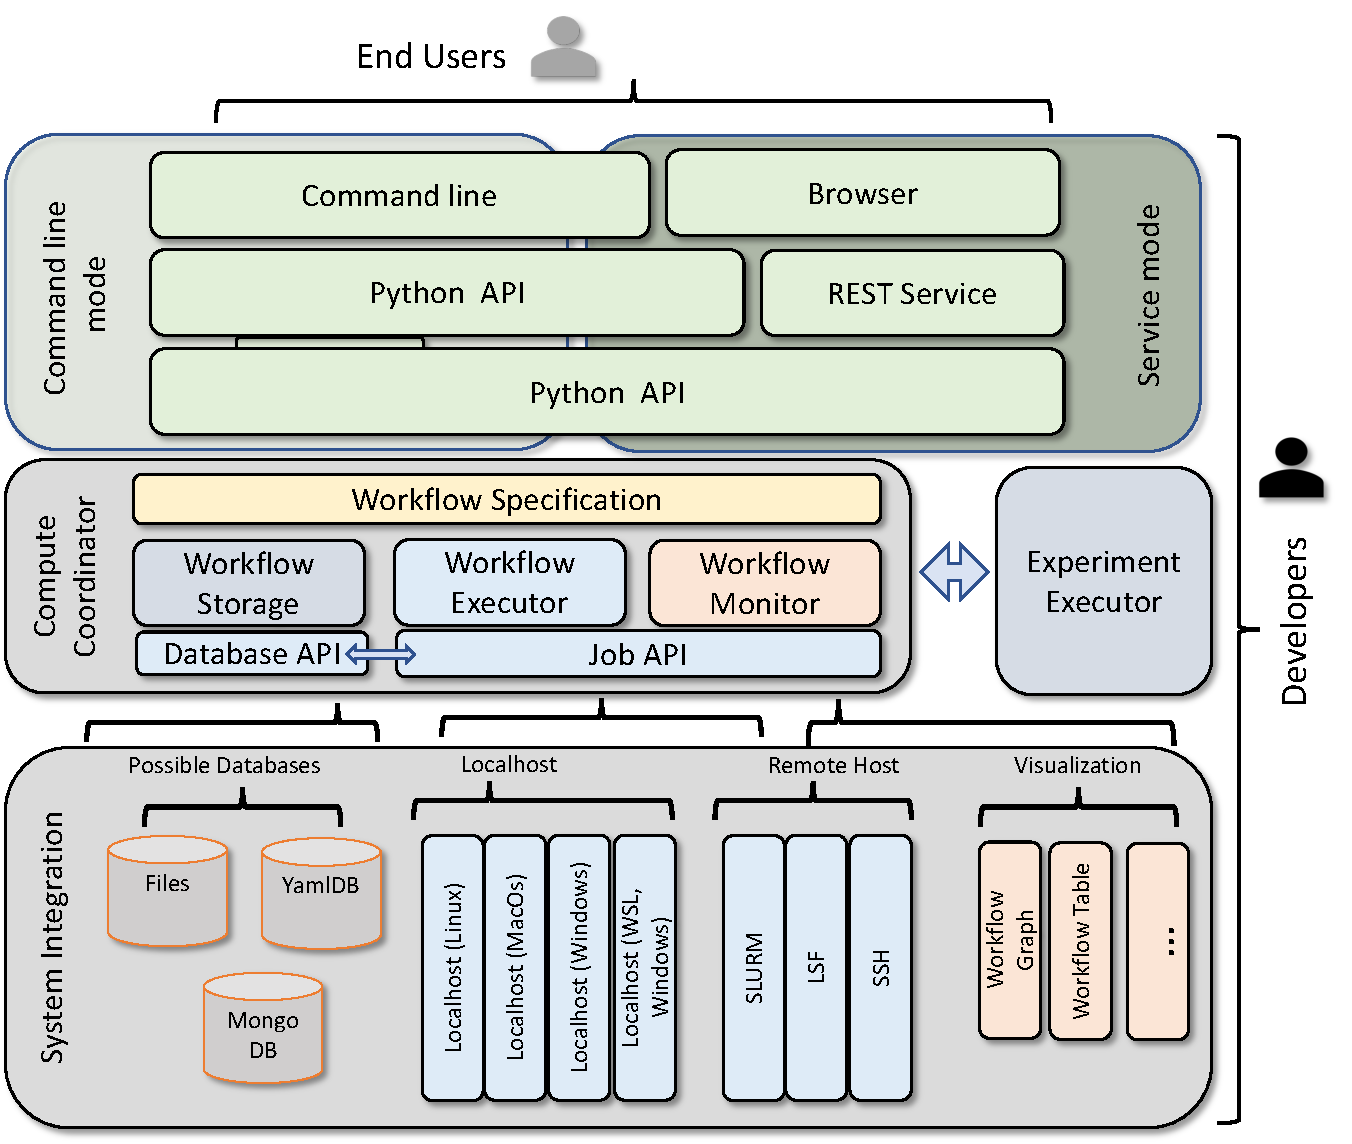
\includegraphics[width=1.0\columnwidth]{images/cloudmesh-cc-arch.pdf}
\vspace{-0.7cm}
\caption{Architecture of the Framework}\label{fig:arch}
\vspace{-0.5cm}
\end{figure}

The framework is based on a layered architecture so that it can be improved
and expanded on at each layer targeting developers and end users.
For the end user, we provide a command line and an intuitive browser interface.  
To support developers, we have designed a 
Python API that is also used to implement a REST Services-based on OpenAPI.

\subsection{Overview of the Task-based Workflow with the Compute Coordinator}

The workflow specification plays an important role in not only
defining a workflow but also in simplifying status updates that are updating an instantiation of a workflow. 
As we have completely separated the status of the
workflow from obtaining status updates, the system allows it to be shut down while the underlying jobs as part of the system integration can still be executed. Once the system is started again it self synchronizes its status from the system integration services. To summarize, the
client is stateless and fetches the state of the submitted
jobs on demand. It will return the latest state found on the job
execution services.

The workflows are defined with human-readable YAML and can be stored in various formats on databases such as Cloudmesh
YamlDB \cite{cloudmesh-yamldb}, which is file-based and provides the easiest integration.
Hence, it is easy to create a variety of monitoring components (for example, as part of a Web
browser) to display the Workflow and its status as a graph, table, or even as a continuous log file. 

One of the most important parts of the framework is how we manage jobs
and monitor their status through a status specification. For this, we have introduced an abstract job
class that is integrated into a workflow class. The job class can
define jobs, start them, and cancel them, to name only the most
important management methods. However, each job defines a status file
in which the actual progress of the job is recorded. This status file
is managed on the compute resource where the job is run and is queried
on demand to return the status to the client. This way, the status of
all jobs can be monitored. As our goal is not to run jobs that execute
in milliseconds but rather in the second range, such status reporting
and propagation is well-suited for us as our tasks are typically long-running.
Our status progress update specification is universally
applicable fia integration into notifications through files (including stdout and stderr) and thus can be issued by bash scripts, SLURM scripts, Python programs, Jupyter
notebooks, or any other computing language.
The workflow status updates are implicitly augmented with timestamps, the compute resource, where it is resulting from, and additional messages to be sent to the monitoring component.
Obviously, the workflow allows the specification of dependencies between tasks.

The framework is managed through a number of open-source repositories in GitHub \cite{github-cloudmesh-ee,github-cloudmesh-ee} and
uses Python as the implementation language. The code is compatible
with Windows, macOS, and Linux.

\subsection{Specifying Task-based Workflows}
\label{sec:task-workflow}

The workflow definition for Cloudmesh is rather simple and intuitive.
An example is provided in Figure~\ref{fig:workflow-example} that specifies a task graph
with the tasks ($start \rightarrow f\!etch\!-\!data
\rightarrow compute \rightarrow analyze \rightarrow end$) representing a typical minimalistic use case for Deep Learning (DL). In this
example the
workflow executes three scripts ([fetch-data,compute,analyze].sh).  Dependencies can easily be specified in human-readable format while using the node name. The nodes contain easy-to-manage information such as the name of the node, a label that is used to print the node's progress, and can contain templated variables such as any value defined as part of a particular node, or specially formatted time stamps. To demonstrate the easy use our label contains the {\em name} and {\em progress} of the workflow which is rendered by the graph or table monitoring components. One can also use variables accessible from Python including operating system or batch system variables to name only a few. Selected examples of values usable in the nodes are listed in Tables~\ref{tab:node-attributes} and \ref{fig:labels-list}. 

\begin{comment}
As the labels and styling are simple to use but have a powerful impact 


The node attributes are listed and summarized 
in
Table~\ref{tab:node-attributes}, while details about the labels are listed in Table \ref{fig:labels-list}. As the labels and styling are simple to use but have a powerful impact on the display of the workflow, we document some of its features in the next sections.
\end{comment}

\begin{figure}[htb]
\vspace{-0.4cm}
{\tiny 
\begin{lstlisting}[breaklines=true]
(*\bfseries workflow:*)
  (*\bfseries nodes:*)
    start:
       name: start
    fetch-data:
       name: fetch-data
       user: gregor
       host: localhost
       status: ready
       label: '{name}\nprogress={progress}'
       script: fetch-data.sh
    compute:
       name: compute
       user: gregor
       host: localhost
       status: ready
       label: '{name}\nprogress={progress}'
       script: compute.sh
    analyze:
      name: analyze
      user: gregor
      host: localhost
      status: ready
      label: '{name}\nprogress={progress}'
      script: analyze.sh
    end:
       name: end
  (*\bfseries dependencies:*)
    - start,fetch-data,compute,analyze,end
\end{lstlisting}}
\vspace{-0.4cm}
\caption{Workflow YAML Configuration file.}\label{fig:workflow-example}
\label{fig:yaml-file}
\end{figure}

\begin{table}[htb]
\centering
\caption{Node attributes.}\label{tab:node-attributes}


{\fontsize{6pt}{6pt}\selectfont
\begin{tabular}{|p{1cm}|p{6.5cm}|}
\hline
{\bf Attribute} & {\bf Description} \\
\hline
\hline
name &  A unique name of the job, must be the same as defined in the : line \\
\hline
user &  The username for the host \\
\hline
host &  The hostname \\
\hline
kind &  The kind of the job, which can be local, ssh, wsl, or slurm  \\
\hline
status &  The status of the job in integer value between 0 and 100 \\
\hline
label &  A custom-designed label \\
\hline
script &  The script name to be executed \\
\hline
\end{tabular}
}

\bigskip

\caption{List of possible labels for nodes on the graph.}
\label{fig:labels-list}

\begingroup

{ \fontsize{6pt}{6pt}\selectfont
  \begin{tabular}{|p{3cm}|p{4.5cm}|}
    \hline
    {\bf Name} & {\bf Description} \\
    \hline
    \hline
    progress &  progress of job from 0-100 \\
    \hline
    now & current time \\
    \hline
    now.\verb|%Y%m%d,%H--%M--%S| &
   now in particular format (this can be used for other times as well) \\
    \hline
    created & time when workflow was created \\
    \hline
    t0.\verb|%Y%m%d,%H--%M--%S| &  workflow start time \\
    \hline
    t1.\verb|%Y%m%d,%H--%M--%S| & workflow end time \\
    \hline
    dt0.\verb|%Y%m%d,%H--%M--%S| & elapsed time since workflow began \\
    \hline
    dt1.\verb|%Y%m%d,%H--%M--%S| & total time of workflow once complete \\
    \hline
    tstart.\verb|%Y%m%d,%H--%M--%S| & job start time \\
    \hline
    tend.\verb|%Y%m%d,%H--%M--%S| & job end time \\
    \hline
    modified.\verb|%Y%m%d,%H--%M--%S| & job modified time \\
    \hline
    os. & operating system environment variable (like os.HOME) \\
    \hline
    cm. & Cloudmesh variable that is read from \verb|cms set| \\
    \hline
\end{tabular}
}
\vspace{-0.5cm}
\endgroup

\end{table}

Other features can also be passed along and may depend on the supporting underlying visualization framework.  in our case, we have provided the ability to also adjust, the node style, color, font, and other to us available display parameters. 

\begin{comment}
\subsection{Node labels}

One particular useful attribute is that of a label. If no label is
used, the name of the node is used as the label. However, if a label
is specified, one can use attribute names and timers to create
labels with implicit state information. This is done by introducing
variables through curly braces. This is of special interest as our DL benchmarks may run a long time and we may want to monitor the progress. 
Table~\ref{fig:labels-list} shows the many useful time-based names one can use in a label. When such a name is used, it can also specify the format of the timer as indicated in an example in the table that shows the default format.

\subsection{Shapes and Styles}

Presently, we use Graphviz \cite{www-graphviz} for rendering the workflow. Thus we also integrated the ability to define attributes provided by Graphviz such as shapes and styles. The full palette of Graphviz features in regard to shapes and styles is supported.

\subsection{Reporting Progress}\label{reporting-progress}

When running jobs inside a Cloudmesh workflow, the called scripts can use a standard format provided by 
{\em cloudmesh.progress} to notify the user and the
backend client monitoring system. This is available in Python, shell, and any other framework as it can be implemented using a write to STDOUT. Such progress is augmented by an integer which indicates 0-100\% progress.
A trivial example encapsulating a machine learning program is shown next.

% {\scriptsize
\begin{lstlisting}[style=sh]
  echo "# cloudmesh status=running progress=1 pid=$$"
  singularity exec --nv ./cloudmask.sif cloudmask.py --config config.yaml 
  echo "# cloudmesh status=done progress=100 pid=$$"
\end{lstlisting}
% }
\end{comment}

How easy it is to integrate the task framework into a Python script using our Cloudmesh StopWatch class and progress method is shown in Figure~\ref{py-api}.
Figure \ref{fig:gui-view} shows the table and graph view of a possible cloudmask workflow. During execution, the information in the views will be automatically updated through server-sent events.
Additional details of these APIs go beyond the purpose of this document and are summarized in \cite{las-22-arxiv-workflow-cc}.

%For Python scripts and Jupyter notebooks, a built-in function is provided as shown next.

\begin{figure}[htb]
\vspace{-0.5cm}
% {\fontsize{6pt}{6pt}\selectfont
{\tiny
\begin{lstlisting}[style=python]
  from cloudmesh.common.StopWatch import progress
  filename = './cloudmesh-log-file.log'
  Stopwatch.start("total")
  progress(progress=1, filename=filename)
  # ... execute your analysis here ...
  progress(progress=100, filename=filename)
  Stopwatch.end("total")
  Stopwatch.benchmark() # prints the benchmark results
\end{lstlisting}
}
\vspace{-0.4cm}
\caption{Python API progress monitoring.}
\label{py-api}
\end{figure}

%Obviously, such progress can be embedded in tools such as tqdm to automatize the logging and help trivial integration with the sophisticated Python ecosystem. 


\begin{comment}
\subsection{Generating Progress Image as Graph}

The framework has a built-in capability to visualize and export the progress of the
workflow in a DAG.

In Figure~\ref{fig:workflow-process}, we depict a simple example
of a workflow that shows the progression of the status over time. Such simple visualization naturally helps to communicate the status and showcases it in the context of the entire workflow. This is often far superior to just monitoring log entries in a file.

\begin{figure}[htb]
\resizebox{1.0\columnwidth}{!}{
\begin{minipage}[b]{0.18\textwidth}
Definition and start \\
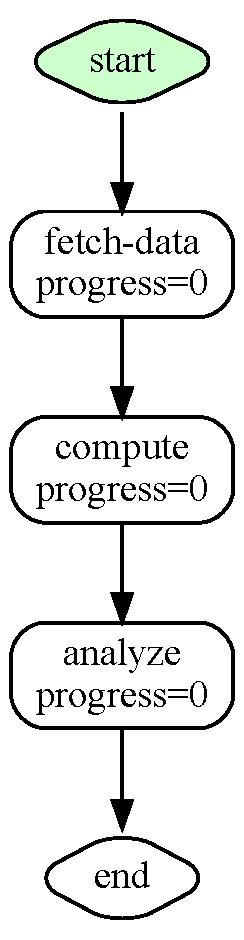
\includegraphics[height=9cm]{images/workflow-example-1.pdf}
\end{minipage} \ \
\begin{minipage}[b]{0.18\textwidth}
Running 1st task \\
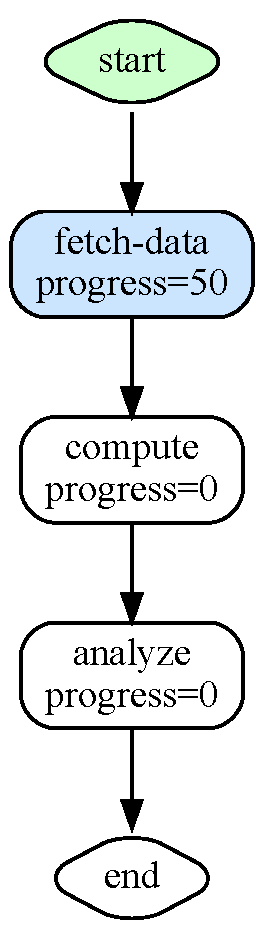
\includegraphics[height=9cm]{images/workflow-example-1.5.pdf} 
\end{minipage} \ \
\begin{minipage}[b]{0.18\textwidth}
Complete 1st task \\
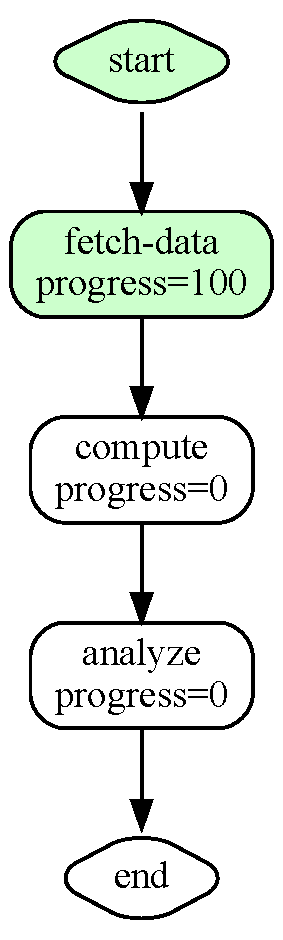
\includegraphics[height=9cm]{images/workflow-example-2.pdf}
\end{minipage} \ \
\begin{minipage}[b]{0.18\textwidth}
Complete 2nd task \\
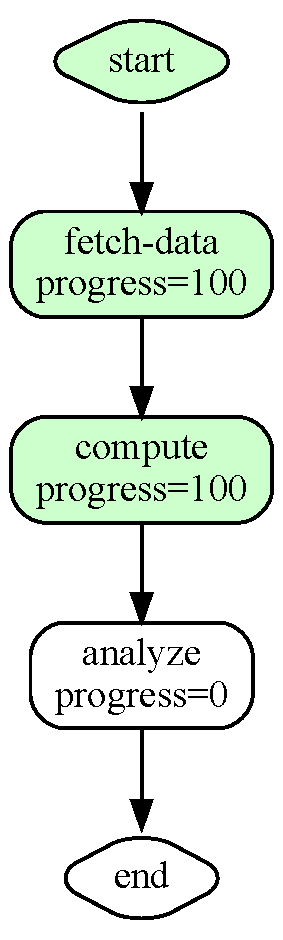
\includegraphics[height=9cm]{images/workflow-example-3.pdf}
\end{minipage} \ \
\begin{minipage}[b]{0.18\textwidth}
Complete workflow \\
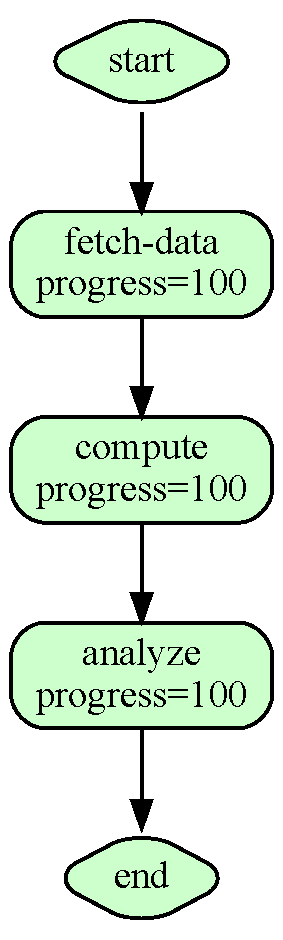
\includegraphics[height=9cm]{images/workflow-example-5.pdf}
\end{minipage} 
}
\caption{The gradual process of a simple workflow.}\label{fig:workflow-process}
\end{figure}

\end{comment}

\begin{comment}

\section{Cloudmesh-cc Interfaces}
\label{sec:cloudmesh-cc-interfaces}



In this section, we explain the various ways of interfacing with the workflow which is distributed in a Python package 
{\em cloudmesh-cc} that includes all but the lower level of our design (see Figure~\ref{fig:arch} and the experiment executor which is implemented in a package called {\em cloudmesh-sbatch}). Interfaces to compute resources are, by design, able to be added via simple pip installs and (once installed through dynamic loading) integrated into the cloudmesh framework instantiation.

It is important to note that we also have a {\em command line mode} that interfaces directly with the backends while not requiring a service. All features are available as Python API. In addition, we have used this API to implement a {\em service}, allowing us to stand up a REST service and a GUI that can be accessed through a Web browser.
Please note that the service mode can also be accessed through the command line
in a terminal and native tools to display the workflow. 
We will now discuss these interfaces in more detail and also showcase
how we can access them.
To support direct execution on the command line, we also provide a command line interface and leverage the cloudmesh command shell, enabling us to interact with the system from the cloudmesh shell on-demand. 

Hence, our work can be integrated into many other frameworks or tools, some of which are listed in the Related Research section. Details of these APIs go beyond the purpose of this document and are summarized in \cite{las-22-arxiv-workflow-cc}.

In addition to the aforementioned interfaces, we also provide a simple Web GUI interface that allows a workflow to be administered and monitored through the GUI. At this time, it contains all the needed functionality to execute and monitor a workflow through a Web browser.

\end{comment}



\begin{figure*}[htb]
\vspace{-0.5cm}
\begin{minipage}[t]{0.99\columnwidth}
\centering  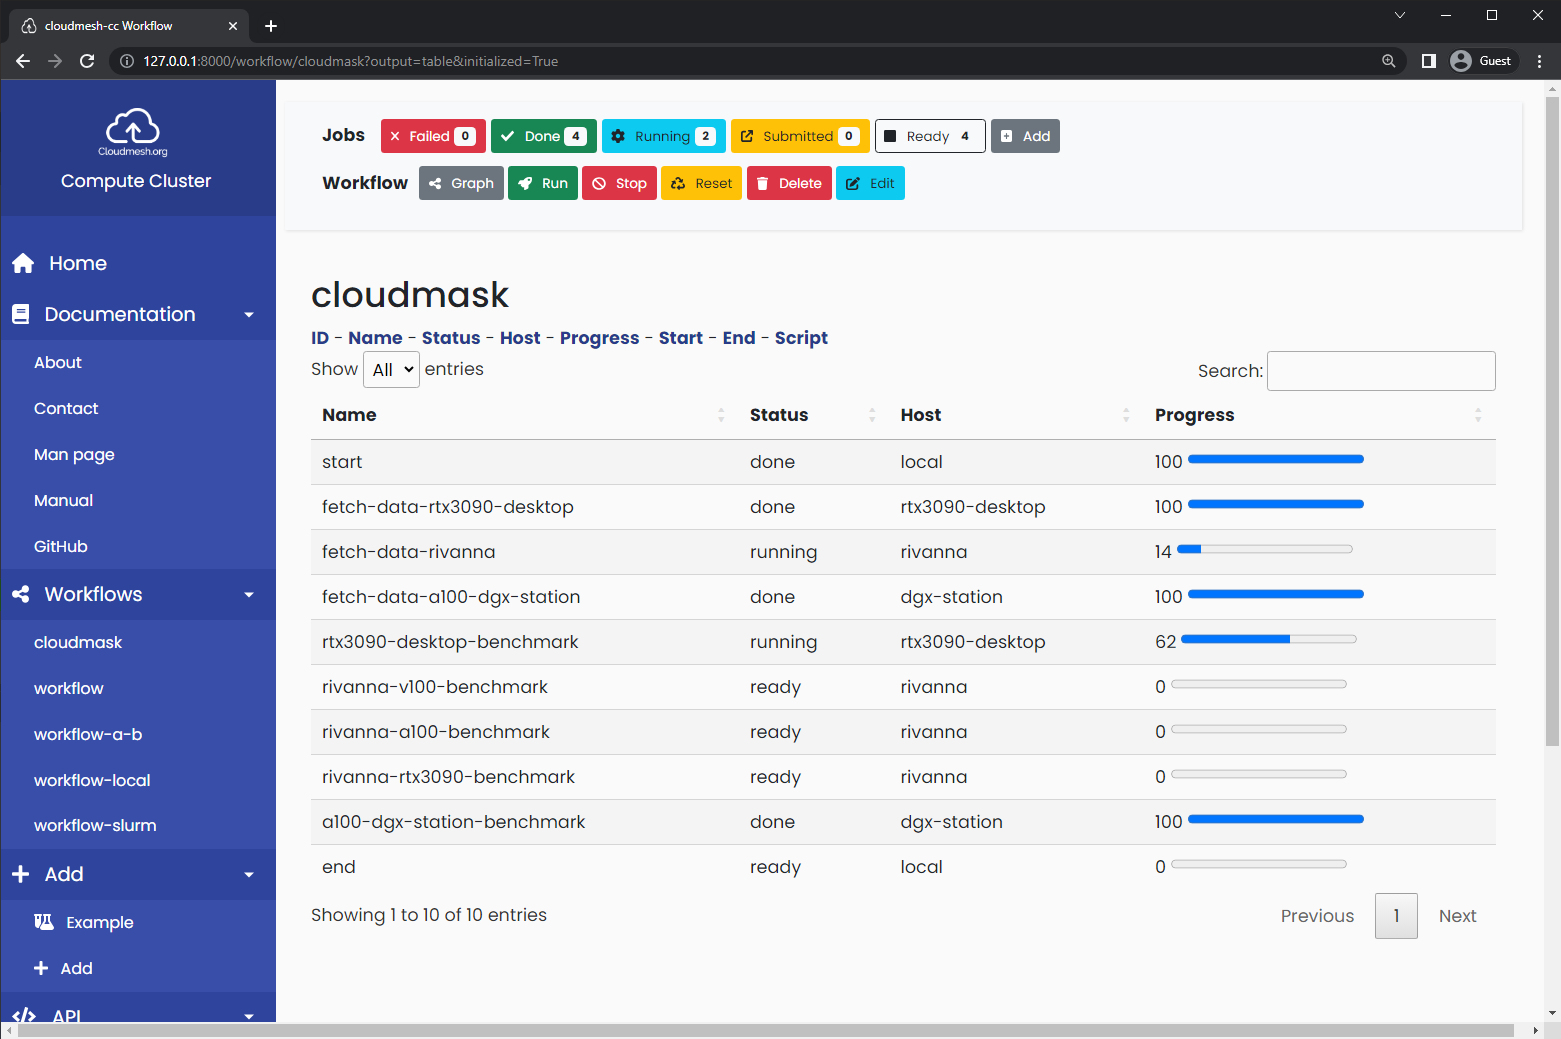
\includegraphics[width=1.0\columnwidth]{images/table-cloudmask-workflow.png}
%\caption{Table view.}
%\label{fig:table-view}
\end{minipage}
\hfill
\begin{minipage}[t]{0.99\columnwidth}
  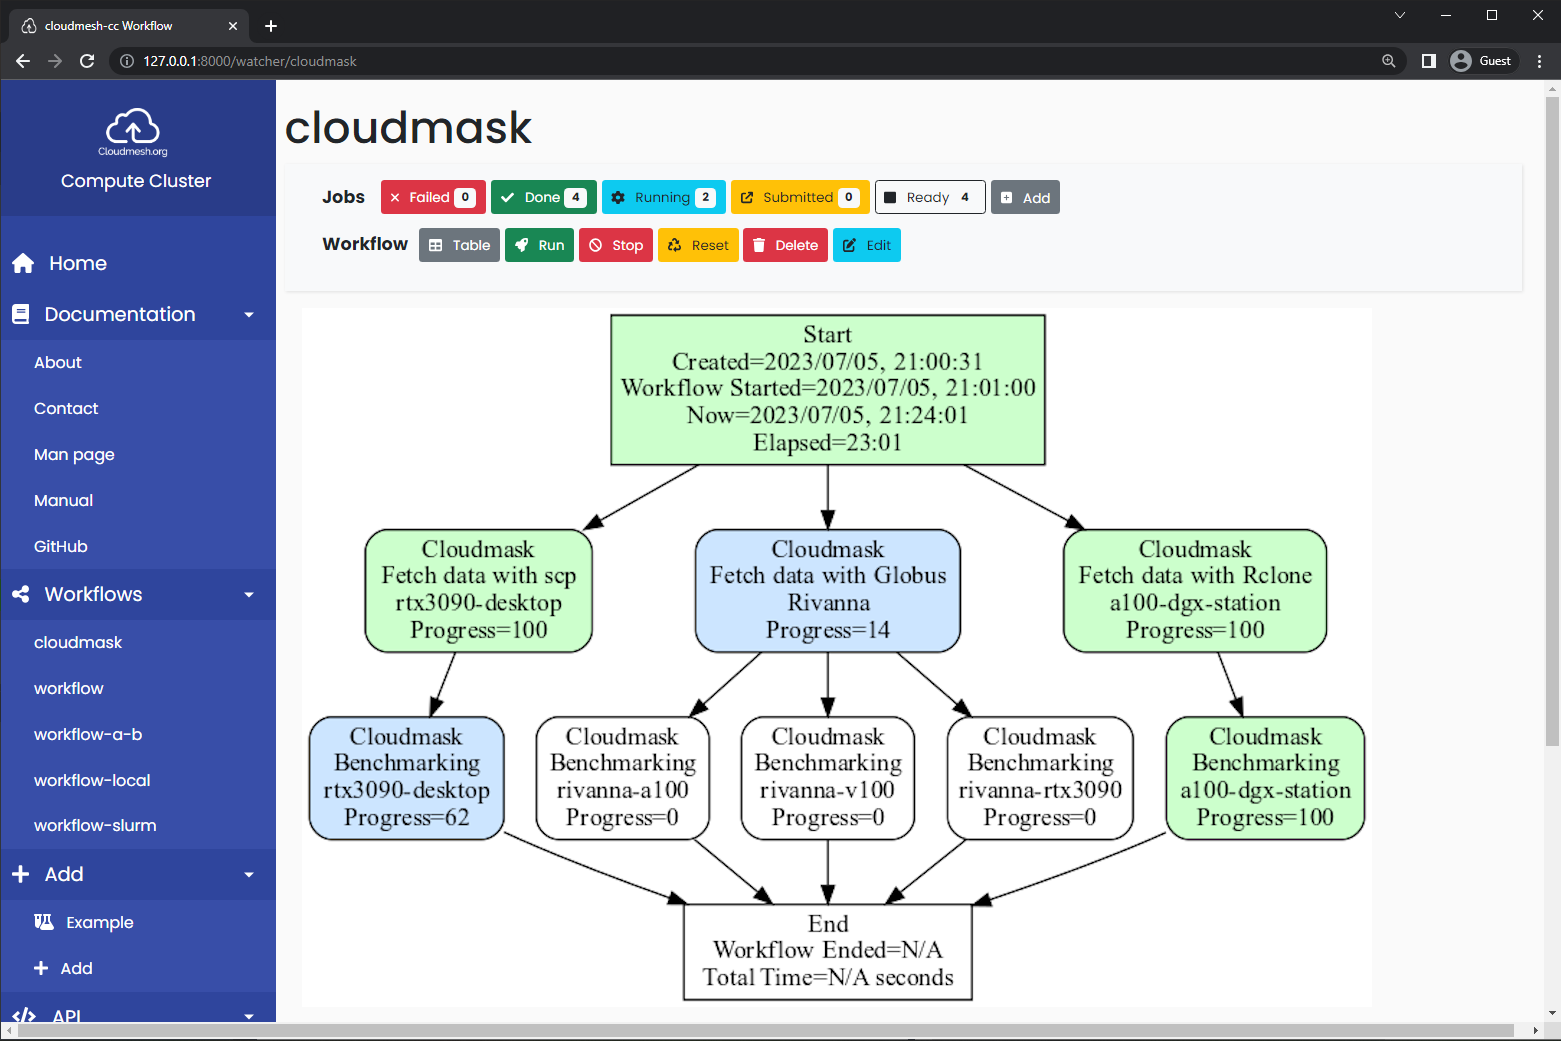
\includegraphics[width=1.0\columnwidth]{images/gui-cloudmask-workflow.png}
\end{minipage}
 \caption{Table and Graph view. Please zoom in for more details.}
\label{fig:gui-view}
\vspace{-0.5cm}
\end{figure*}


\begin{comment}
\subsection{Cloudmesh-sbatch}
\label{sec:cloudmesh-sbatch}

\begin{figure}[htb]
    \centering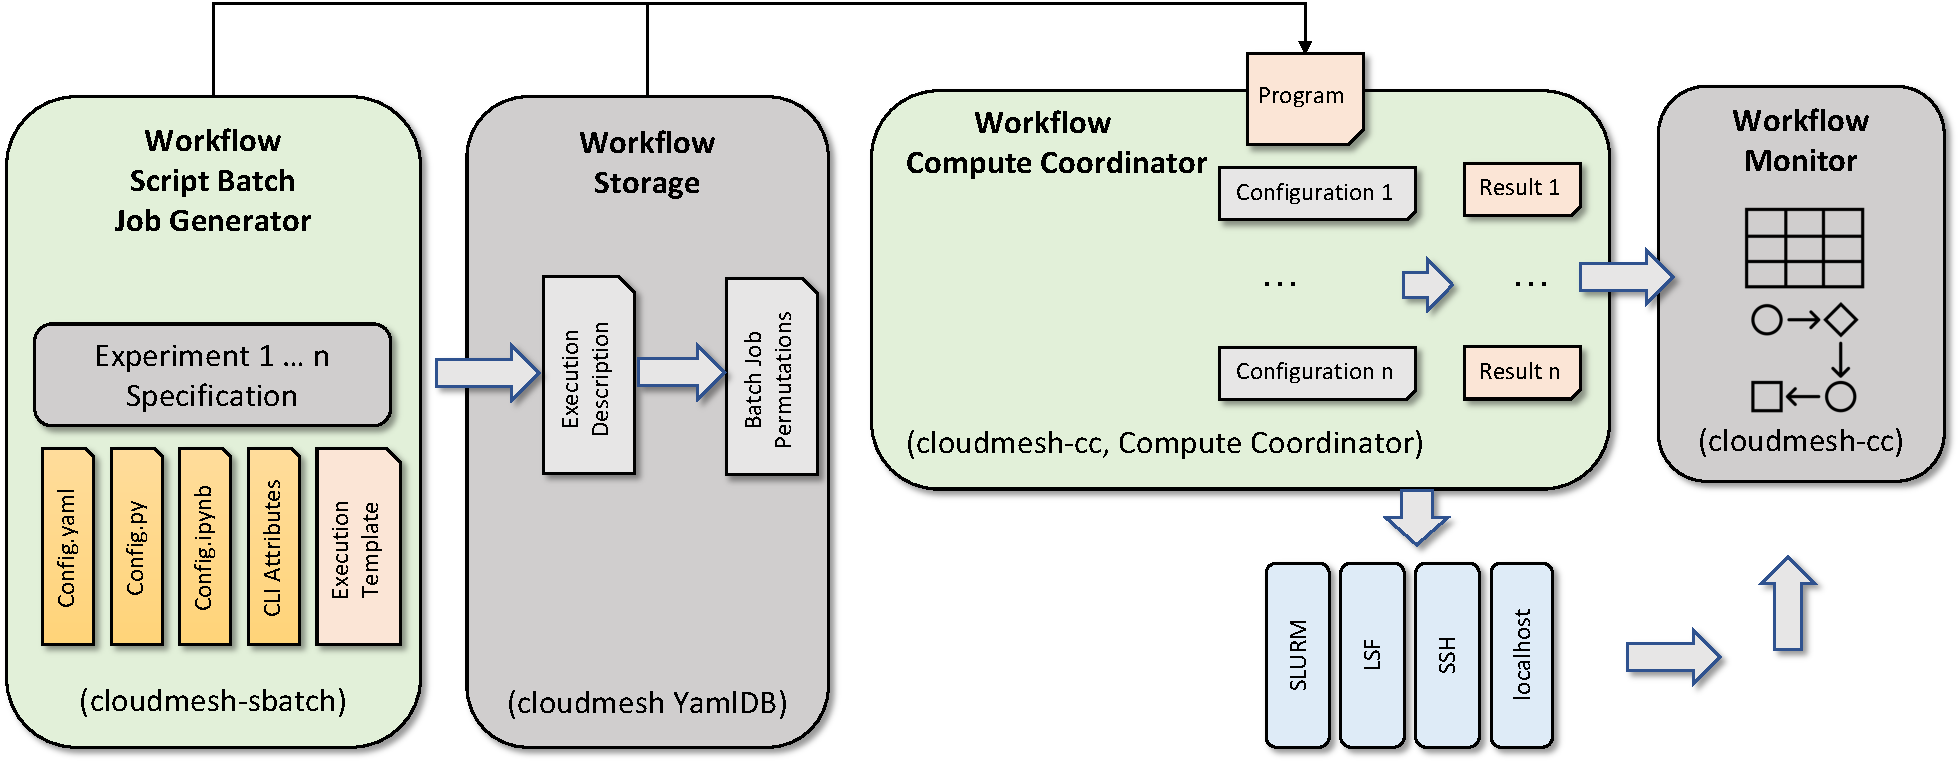
\includegraphics[width=1.0\columnwidth]{images/cloudmesh-sbatch-new}
    
    \caption{Experiment management workflow architecture design of cloudmesh-sbatch.}
    \label{fig:cc-2}

\end{figure}
\end{comment}

\subsection{Experiment Execution}
\label{sec:workflow-sbatch}

It is important to note that the system not only includes a task workflow system but also allows the execution of iterations over experiment parameters as used in identifying optimal parameter sets maximizing for example the accuracy of a scientific application. The component to coordinate this is called {\em Experiment Executor} (EE). In traditional machine learning workflows, hyperparameter tuning and configuration are key elements in assessing and optimizing the performance of models. However, scaling hyperparameters for highly parallel execution with heterogeneous hardware is complex. The EE can be used to generate many parameter settings including the utilization of the type of GPU or the system hardware on which the experiment is executed. In Figure \ref{fig:gui-view} we showcase the execution of an experiment that combines the Cloudmesh components of CC and EE to find the best accuracy across a number of different compute resources and GPUs. The EE jobs can utilize various queuing systems such as SLURM, and LSF, but also sequential and parallel ssh jobs. The scheduling of the jobs to be executed could be customized. For our simple example, we provide a simple Cartesian product for all experiment parameters provided. The advantage of this system is through the templated configuration files steering the application, quick adaptations can be made to identify more suitable hyperparameter settings. Furthermore, the use of the system implicitly promotes the reaction of a unique directory for each experiment in which the executed program and its output are stored. This fosters reproducible experiments following the FAIR principles 
As the structure of the experiment is including the hyperparameter settings, results from different computing systems can be merged into the overall results. Thus the EE supports the creation of coordinated results while allowing the generation of cooperating, selective, and distributed result generation. A simple experiment configuration file is showcased next, where we execute a scientific application called cloudmask for epochs 1, 30, and 60, on the GPUs v100 and a100 repeating it 5 times.

{\scriptsize
\begin{lstlisting}[breaklines=true]
    application:
        name: cloudmask
    data: "/scratch/{os.USER}/{application.name}"
    experiment:
        epoch: "1,30,60"
        gpu: "a100,v100"
        repeat: "1,2,3,4,5"
\end{lstlisting}
}

Dependent on the queuing system a custom templated batch script utilizing these variables is created and used during the experiment execution. As it is templated and user-independent, it can then also be executed via different user accounts, either separately, or jobs being split up across different user accounts. An additional benefit from our templated executions is that an energy monitor can be integrated creating energy traces throughout the calculation. This helps as we can also compare and predict the energy consumption for long-running jobs which is of considerable importance due to the overall resources consumed by many scientific deep learning applications. Furthermore, we developed the best practice to predict for deep learning applications the computational and storage needs base on a few hyperparameter combinations so that planing can take place to acquire sufficient resources for long running templated experiments.

While practically working with the system, we observed that students (as part of research experiences) not using our experiment executor spend a significant amount (weeks-months) of a semester on setting up a benchmark and replicating only a fraction of the functionality provided by the EE. However, we tested the system out while other students used EE and we observed that the applications for which a template and configuration file has been designed reduced the on-ramp time to less than a day.

\section{Other Cloudmesh Features}
\label{sec:cloudmesh-other}

Cloudmesh has its origin in supporting various cloud computing resources, making it easy to develop and integrate them into the execution workflow to set up and use cloud resources as computational resources. It provides AWS, Azure, Google, and OpenStack cloud interfaces for virtual machine and data file services. Cloudmesh was the first tool that developed as a hybrid cloud
API, command line, and command shell framework.  As it uses templated virtual machine specifications, it is easy to switch from one cloud to another with a one-line command.
Other services include the automated generation of REST services from Python APIs as documented~\cite{las21-gas}.

For benchmarking, Cloudmesh also automatically exports MLCommons log events but uses the much more sophisticated, intuitive, and easier-to-use Cloudmesh StopWatch, making it possible to export benchmark timers in a human-readable format.
 

\section{MLCommons Cloudmask Workflow}
\label{sec:cloudmask-workflow}

We are applying the CC and EE workflow system to a number of MLCommons and non MLCommons applications \cite{las-22-arxiv-workflow-cc,las-22-mlcommons-science}. However, here we only summarize our experience as applied to the MLCommons Science Group Cloudmask application.

Cloudmask is a program that develops a model to classify sections of
satellite images as either containing clouds or clear skies by using
machine learning \cite{www-cloudmask}. We used CC to coordinate the execution of cloudmask between different systems and EE to execute various parameter settings and iterate over the chosen hyperparameters.
This includes an HPC computer at the University of Virginia called Rivanna, as well as two desktop
computers (Figure ~\ref{fig:gui-view}). As we are able to coordinate the execution of the workflows across different machines and merge the results we were able to easily create a runtime comparison between the different compute resources (see Figure~\ref{fig:runtime-comp}, here shown only for one epoch). 



An automated script has been developed that produces the selected outputs that one usually finds with deep learning parameter studies (\ref{fig:runtime-comp}-\ref{fig:inf-acc-spectrum}). The workflow runs approximately 24 hours while producing the results in parallel on multiple compute resources and multiple GPUS. 

\begin{comment}
\begin{figure*}[htb]
\centering
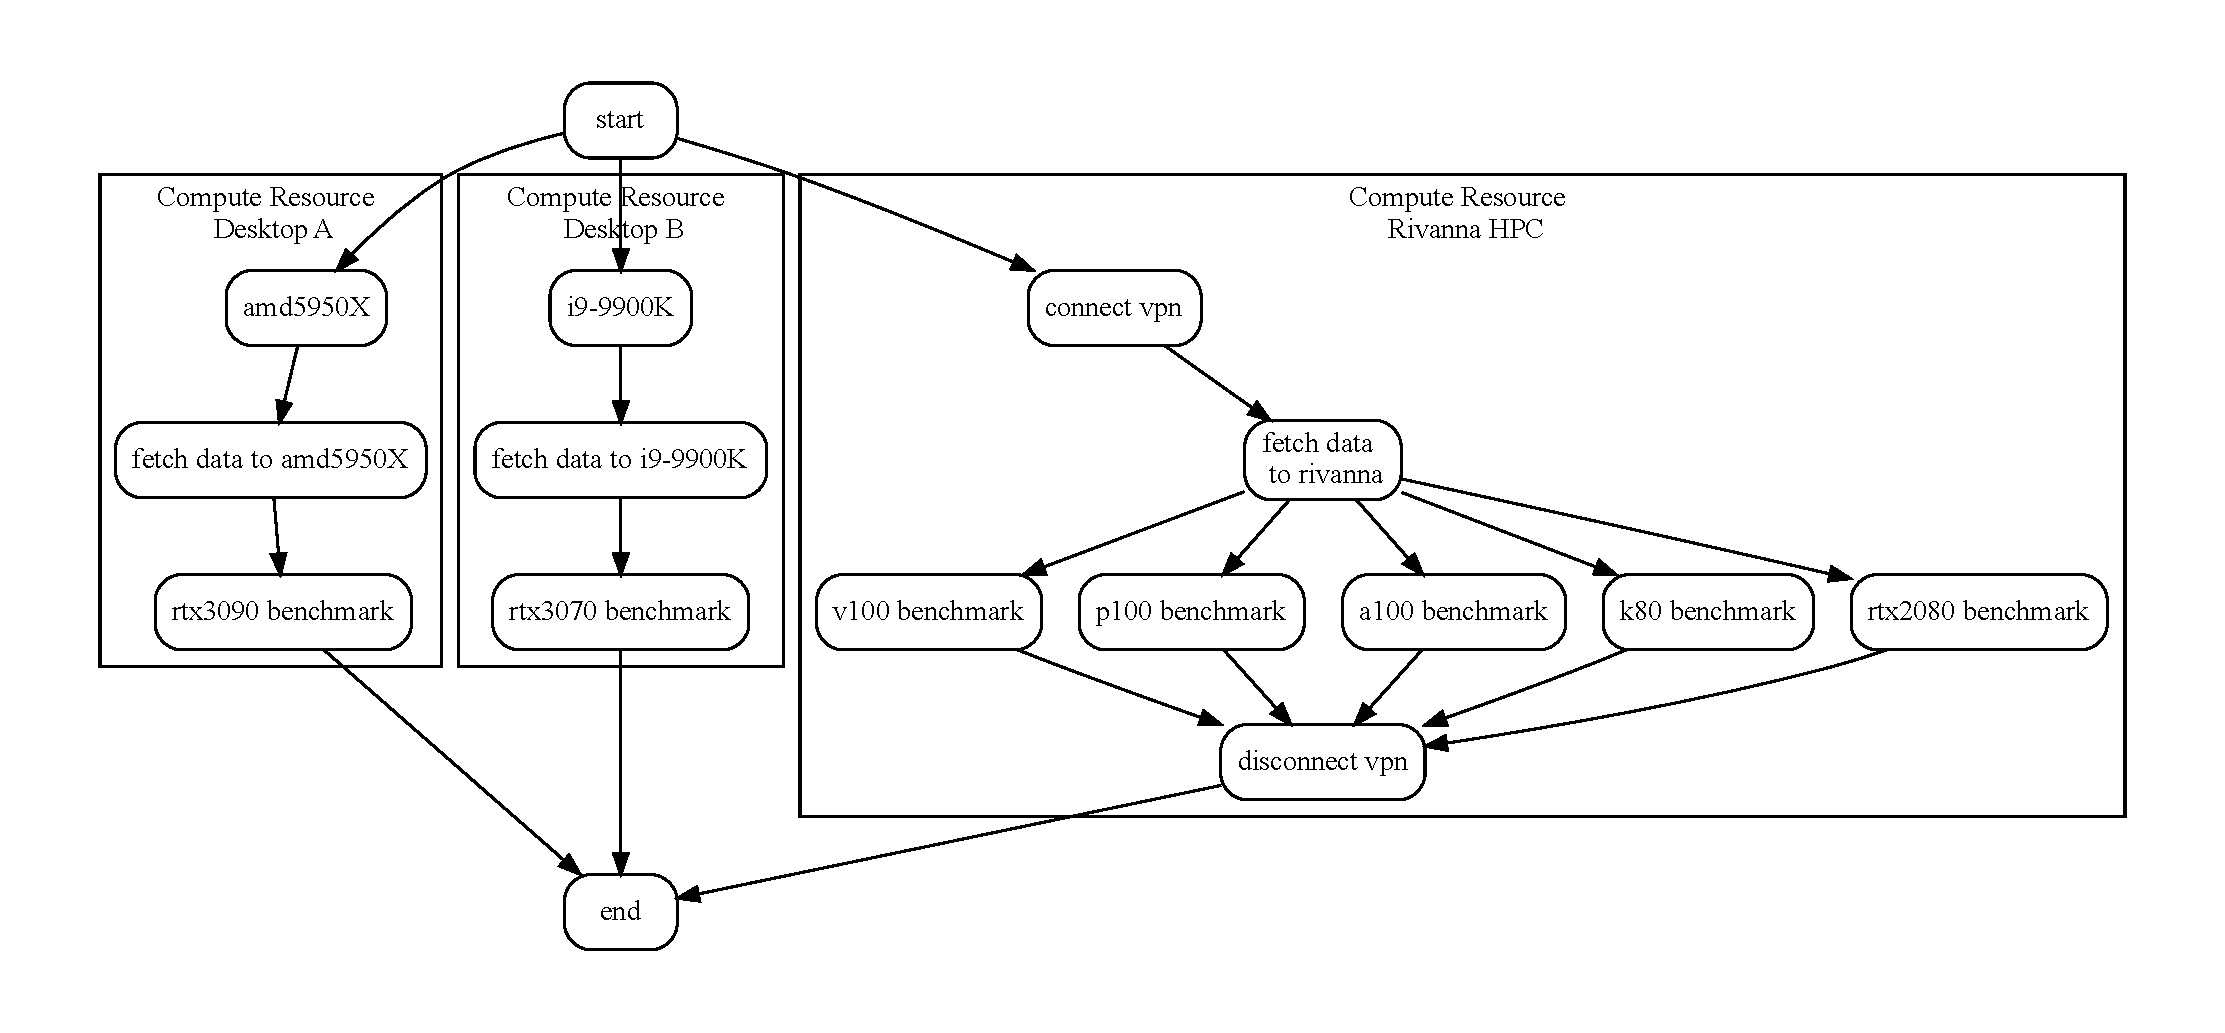
\includegraphics[width=0.75\textwidth]{images/cloudmask-wf.pdf}
%\vspace{-1cm}
\caption{Workflow for Cloudmask}\label{fig:cloudmaskwf}
\end{figure*}
\end{comment}

\begin{comment}
The workflow will take approximately 24 hours to run if resources are
available. The workflow iterates through five GPUs available on
Rivanna, including V100, P100, A100, K80, and RTX2080, and runs the
program three times on each GPU. Each run trains the model with 10,
30, and 50 epochs for benchmarking. Upon completing a run, the logs
and benchmarks are written into a results folder. 
In the following figures, we showcase a subset of the workflow 
to increase readability in this publication production of paper.

All results produced from the various machines can be agglomerated 
into a single analysis directory on which our Jupyter notebook can be run to produce customized outputs.

We showcase in Figures \ref{fig:runtime-comp}-\ref{fig:inf-acc-spectrum} selected templates that we include in our analysis script that can easily be adapted to other applications. It includes 
 benchmark comparisons of Cloudmask between graphics cards
(Figure~\ref{fig:runtime-comp}),
training history validation accuracy
(Figure~\ref{fig:train-hist-val-acc}),
training history validation loss
(Figure~\ref{fig:train-hist-val-loss}),
training history accuracy
(Figure~\ref{fig:train-hist-acc}),
training history loss
(Figure~\ref{fig:train-hist-loss}),
and more.

Additionally for this application, we integrated a custom analysis script that obtains differences in inference accuracy while aligning them with the various samples used for the inference as shown in the Figures titled
Inference accuracy (Figure~\ref{fig:inf-acc}) and
Inference accuracy over sample as a spectrum
(Figure~\ref{fig:inf-acc-spectrum}). The last two images from our workflow especially demonstrate that some training data perform poorly on our trained model for this application. Thus, a further improvement of the application is justified. Having our workflow and the templates as starting points will simplify research into this and other applications that utilize the framework. We are looking forward to an improved version of MLCube, which we will then integrate into this application and also utilize in our toolchain.
\end{comment}


\begin{figure}[htb]
{
\begin{center}
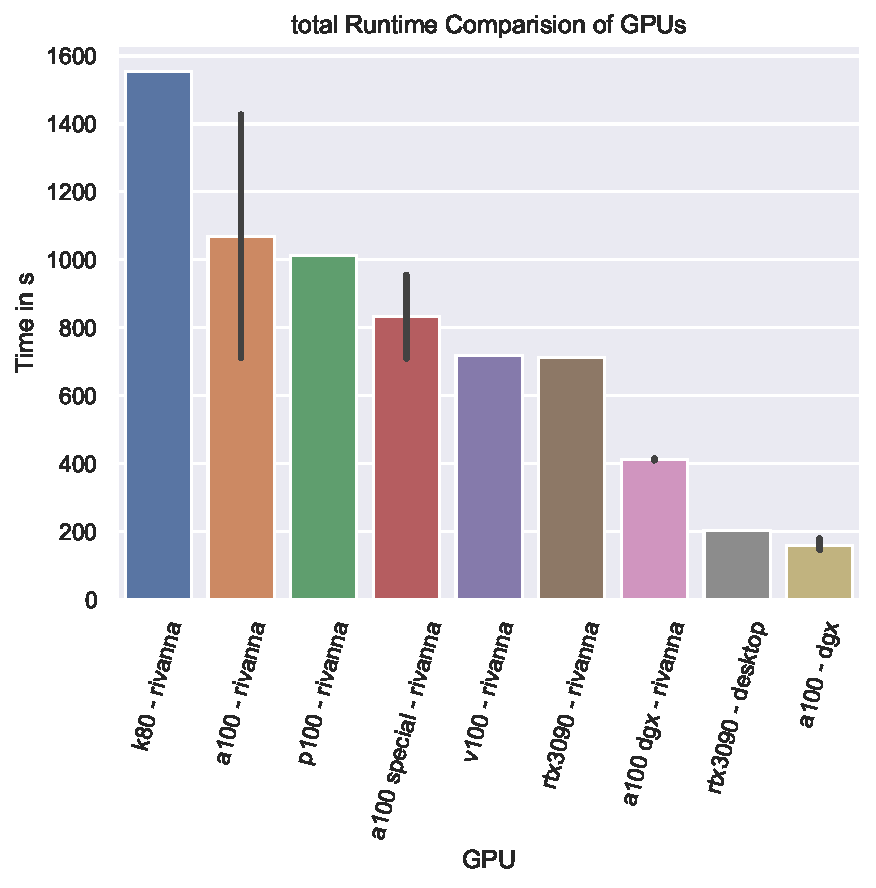
\includegraphics[width=0.85\columnwidth]{images/rivanna-comparision-epoch-1.pdf}
\end{center}
}
\vspace{-0.7cm}
\caption{Runtime comparisons of Cloudmask between graphics cards}
\label{fig:runtime-comp}
\vspace{-0.5cm}
\end{figure}

%%%%%%%%%%%%%%%%%%%%%

\begin{figure*}[htb]

%%%%%%%%%%%%%%%%%%%%%
\begin{minipage}[t]{0.3\textwidth}
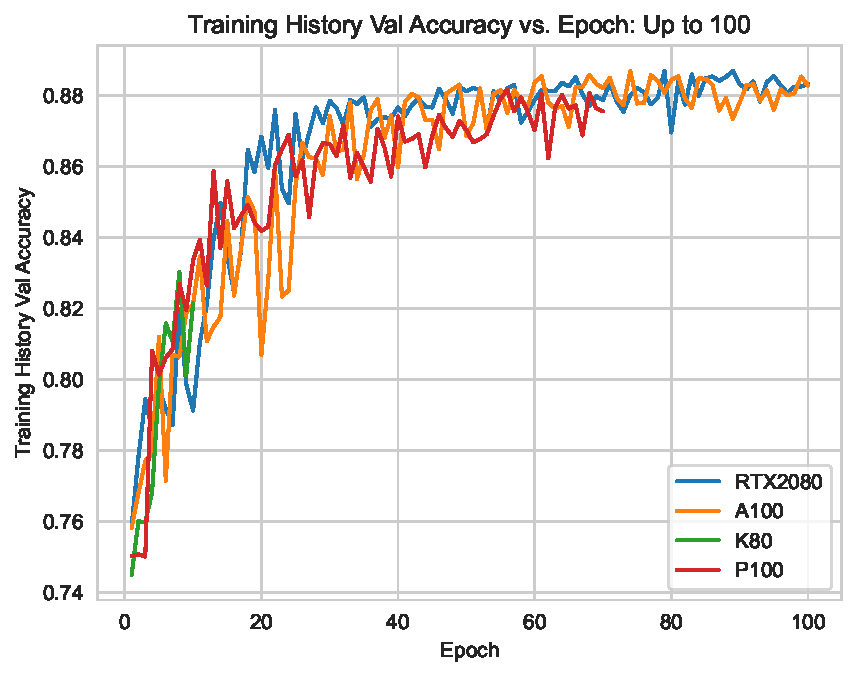
\includegraphics[width=1.0\textwidth]{images/training-history-val_accuracy.pdf}
\caption{Training history validation accuracy}
\label{fig:train-hist-val-acc}
\end{minipage}
\hfill
\begin{minipage}[t]{0.3\textwidth}
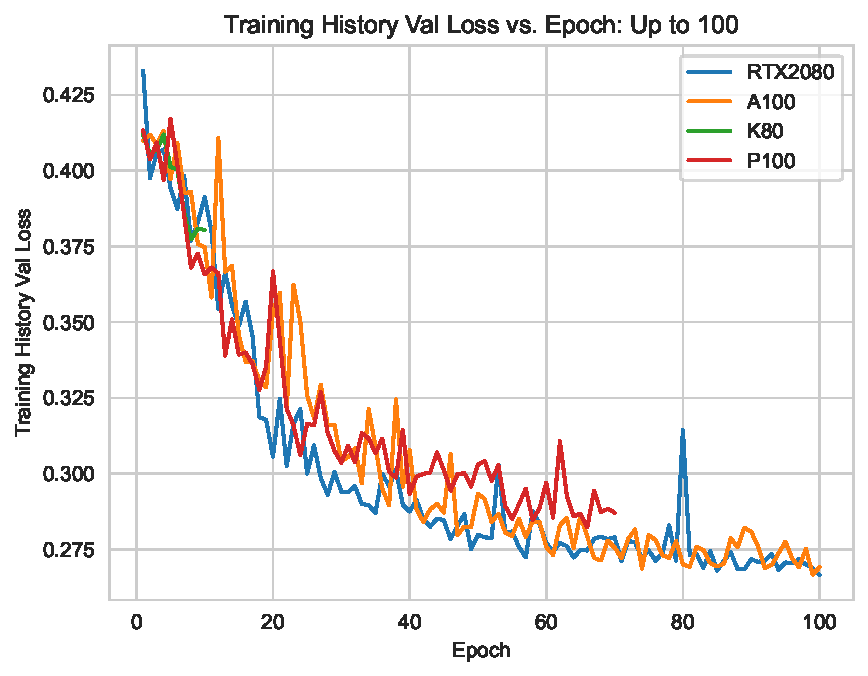
\includegraphics[width=1.0\textwidth]{images/training-history-val_loss.pdf}
\caption{Training history validation loss}
\label{fig:train-hist-val-loss}
\end{minipage}
\hfill
\begin{minipage}[t]{0.3\textwidth}
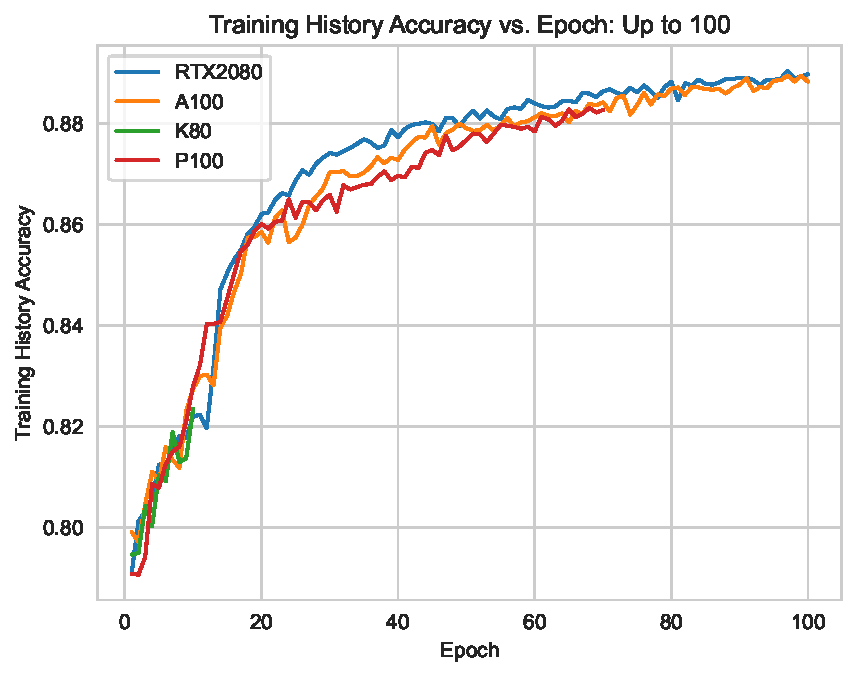
\includegraphics[width=1.0\textwidth]{images/training-history-accuracy.pdf}
\caption{Training history accuracy}
\label{fig:train-hist-acc}
\end{minipage}


\begin{minipage}[t]{0.3\textwidth}
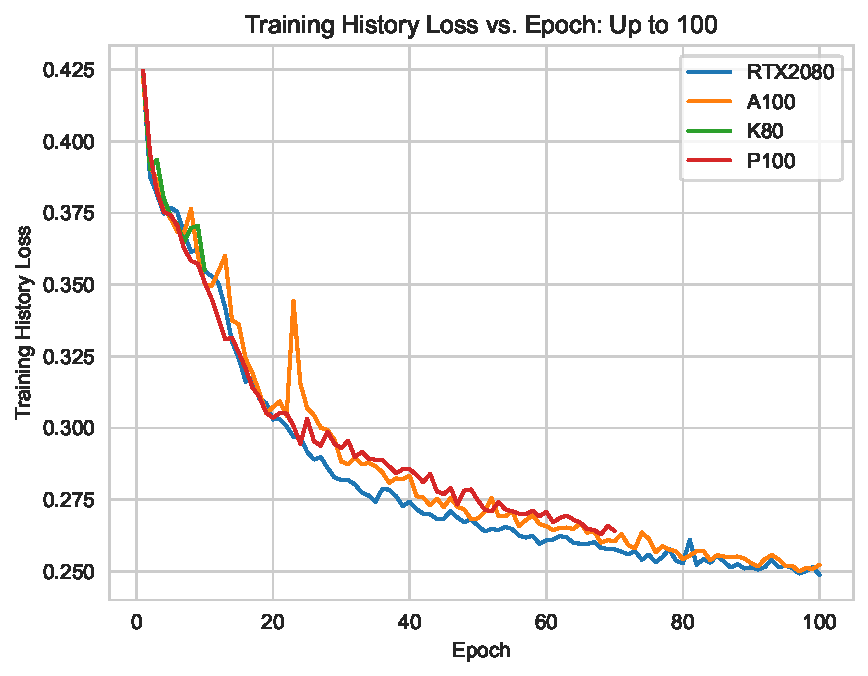
\includegraphics[width=1.0\textwidth]{images/training-history-loss.pdf}
\caption{Training history loss}\label{fig:train-hist-loss}
\end{minipage}
\hfill
\begin{minipage}[t]{0.3\textwidth}
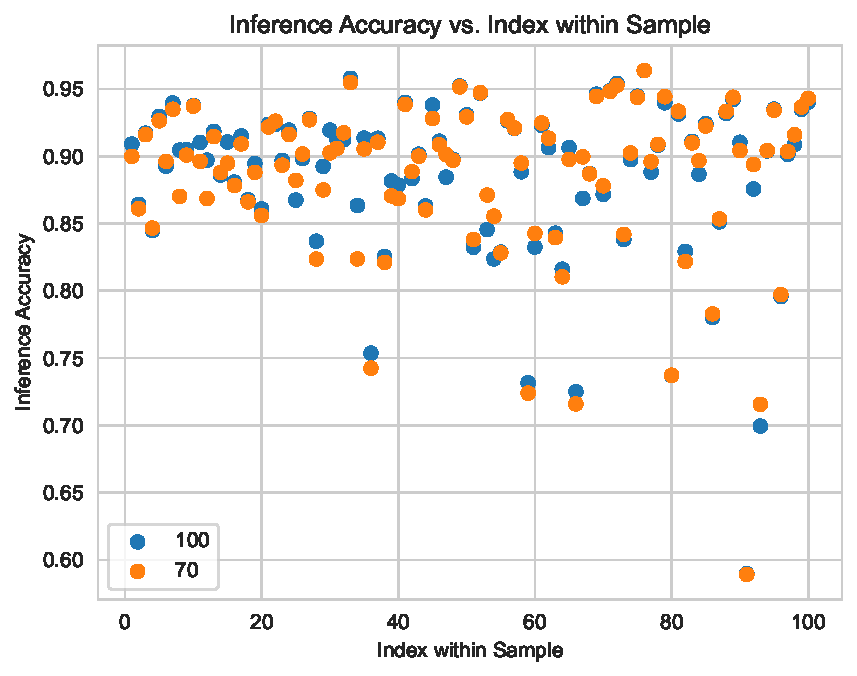
\includegraphics[width=1.0\textwidth]{images/inference-accuracy.pdf}
\caption{Inference accuracy}
\label{fig:inf-acc}
\end{minipage}
\hfill
\begin{minipage}[t]{0.3\textwidth}
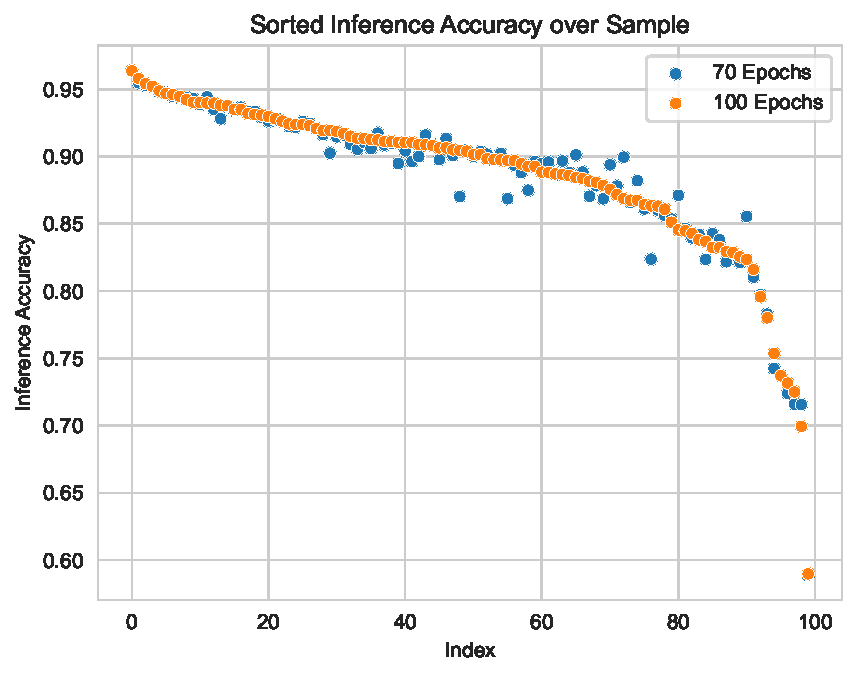
\includegraphics[width=1.0\textwidth]{images/spectrum-inference-accuracy.pdf}
\caption{Inference accuracy over sample as a spectrum.}
\label{fig:inf-acc-spectrum}
\end{minipage}
\vspace{-0.5cm}

\end{figure*}


\section{Conclusion}
\label{sec:conclusion}

We have designed and implemented a Hybrid Reusable Computational
Analytics Workflow Management with the help of the Cloudmesh component
framework. The component added focuses on the management of workflows
for computational analytics tasks and jobs. The tasks can be executed
on remote resources via ssh and even access queuing systems such as
Slurm. In addition, we can integrate the current computer on which the
workflow is running. This can include operating systems such as Linux,
macOS, Windows, and even Windows Subsystem for Linux. Through
Cloudmesh, access to a command line and a command shell is provided. A
simple API and a REST interface are provided. The framework also has
an elementary Web browser interface that allows visualizing the
execution of the workflow. It is important to know that the workflow
can be started on remote resources and is running completely
independently from the client tool once a task is started in contrast to many other workflow systems. This allows
a ``stateless'' model that can synchronize with the remotely started
jobs on demand through pull request. Hence, the framework is self-recovering in case of
network interruptions or power failure eve on the client side. Due to our experiences with
real (and many) infrastructure failures at the authors' locations, the
availability of such a workflow-guided system was
beneficial. Although very large graphs can be created we envision the utilization for graphs between 1 - 1000 nodes. 
 The targeted task based run from minutes to hours and days and the state synchronization is fast in comparison to the runtime of individual tasks.
The developed code is rather small and, in
contrast to other systems, is less complex. The workflow specification and integration of monitoring is easy.
Hence, it is suitable for
educational aspects as it is used for master's and undergraduate-level
research projects to apply the workflow, but also to enhance it. The project has and is practically utilized
while generating benchmarks for the MLCommons Science Working Group
showcasing real-world applicability beyond a student research project. 
Most importantly, the work to execute such benchmarks has been reduced 
from weeks to a day. The framework was first used to unexpectedly discover and report IO latency's while comparing traditional HPC systems with very fast desktops using NVMe's, resulting in recommendations improving the IO storage of the HPC system. Thus the framework not only allows fast on-ramp time for users, but has been used to communicate system related performance issues that since have been improved. Future activities include adaptation to more applications. 

\section*{Acknowledgment}

Work was in part funded by (a)  NIST 60NANB21D151T (a) NSF CyberTraining: CIC: CyberTraining for Students and Technologies from Generation Z with the award numbers 1829704 and 2200409 and NIST 60NANB21D151T (b) Department of Energy under the grant Award No. DE-SC0023452 (c) the Biocomplexity Institute and Initiative at the University of Virginia.  We like to thank the reviewers for their valuable feedback.


\bibliographystyle{IEEEtran}

\bibliography{vonLaszewski-cloudmesh-cc}




\end{document}
\endinput
%%
%% End of file `sample-sigplan.tex'.

